%# -*- coding: utf-8-unix -*-
%%==================================================
%% thesis.tex
%%==================================================

% 双面打印
% \documentclass[doctor, fontset=adobe, openright, twoside]{sjtuthesis}
\documentclass[bachelor, fontset=adobe, openany, oneside, submit]{sjtuthesis}
% \documentclass[master, fontset=adobe, review]{sjtuthesis}
% \documentclass[%
%   bachelor|master|doctor,	% 必选项
%   fontset=adobe|windows,  	% 只测试了adobe
%   oneside|twoside,		% 单面打印,双面打印(奇偶页交换页边距,默认)
%   openany|openright, 		% 可以在奇数或者偶数页开新章|只在奇数页开新章(默认)
%   zihao=-4|5,, 		% 正文字号:小四、五号(默认)
%   review,	 		% 盲审论文,隐去作者姓名、学号、导师姓名、致谢、发表论文和参与的项目
%   submit			% 定稿提交的论文,插入签名扫描版的原创性声明、授权声明 
% ]

% 逐个导入参考文献数据库
\addbibresource{bib/thesis.bib}
% \addbibresource{bib/chap2.bib}

\begin{document}

%% 无编号内容:中英文论文封面、授权页
%# -*- coding: utf-8-unix -*-
\title{基于密钥信息的密钥编排方案评估、优化与设计}
\author{陈\quad{}墨}
\advisor{来学嘉教授}
% \coadvisor{某某教授}
\defenddate{2017年6月7日}
\school{上海交通大学}
\institute{电子信息与电气工程学院}
\studentnumber{5130309203}
\major{计算机科学与技术}

\englishtitle{On the Evaluation, Optimization and Design of Key Schedule based on Key Information}
\englishauthor{\textsc{Mo Chen}}
\englishadvisor{Prof. \textsc{Xuejia Lai}}
% \englishcoadvisor{Prof. \textsc{Uom Uom}}
\englishschool{Shanghai Jiao Tong University}
\englishinstitute{\textsc{Depart of Computer Science and Engineering, School of Electronics, Information and Electrical Engineering} \\
  \textsc{Shanghai Jiao Tong University} \\
  \textsc{Shanghai, P.R.China}}
\englishmajor{Computer Science}
\englishdate{Jun. 7th, 2017}


\maketitle

\makeenglishtitle

\makeatletter
\ifsjtu@submit\relax
	\includepdf{pdf/original.pdf}
	\cleardoublepage
	\includepdf{pdf/authorization.pdf}
	\cleardoublepage
\else
\ifsjtu@review\relax
% exclude the original claim and authorization
\else
	\makeDeclareOriginal
	\makeDeclareAuthorization
\fi
\fi
\makeatother


\frontmatter 	% 使用罗马数字对前言编号
\pagestyle{front}
\begin{bigfront}

%% 摘要
%# -*- coding: utf-8-unix -*-
%%==================================================
%% abstract.tex for SJTU Master Thesis
%%==================================================

\begin{abstract}

分组密码中常常较为简单的密钥编排方案的低扩散程度常常会导致一些密码攻击。
为了描述与量化这种扩散程度以分析和设计密钥编排方案,黄佳琳等人给出了以实际密钥信息(Actual Key Information)为核心的关于密钥信息的一系列概念。
但是,现有的计算实际密钥信息的算法仍处于贪心(只能给出上界)或是简单枚举的阶段,其正确性和效率性的缺乏限制了其只能用于攻击而不能用于分析、设计编排方案。
在本文中,我们成功地解决了AKI问题这一难题,提出了一个基于图论中著名的最大流问题的一个全新的AKI-最小割算法,同时还进一步给出了一个基于该算法的密钥编排设计方法,旨在设计出一个无密钥信息泄露的密钥编排方案来提供更强的安全性。
作为以上算法的应用,我们成功了优化了对23轮TWINE-80密码的多维零相关线性攻击,并提出了一个新的对12轮RECTANGLE-128的中间相遇攻击。
同时,我们针对以上两个密码及其攻击,分别为这两个密码算法优化、设计了新的密钥编排方案,使其能够抵抗上述攻击,甚至相类似的一系列攻击。

\keywords{\large 分组密码\quad 密钥编排方案 \quad 密钥信息 \quad 实际密钥信息 \quad 最大流问题 \quad 图论 \quad AKI-最小割算法\quad TWINE \quad RECTANGLE \quad 密钥编排方案的优化与设计}
\end{abstract}

\begin{englishabstract}

    The low diffusion of a simplified key schedule in block ciphers is usually responsible for many attacks.
    Huang \emph{et al.} gave conceptions on Key Information, especially the Actual Key Information (AKI), which successfully illustrated and quantified the method to evaluate the diffusion of a key schedule.
    However, the algorithm used to calculate AKI proposed by Huang \emph{et al.} cannot be used to determine the weakness or further make an optimization of a key schedule since it cannot give an accurate value of AKI.
    In this paper, we successfully solve the AKI problem by our AKI - Minimum Cut Algorithm based on the well-known Max-flow problem in Graph Theory,
    and futher give a method to design a key schedule which offers better security with less or without Key Information leakage.
    As applications, we optimize the zero-correlation attack on 23-round TWINE-80 and find a new meet-in-the-middle attack on 12-round RECTANGLE-128,
    and respectively gives a new dependency matrix for TWINE-80 and an optimized key schedule for RECTANGLE-128, which makes both of them stronger against these attacks.

\englishkeywords{\large Block cipher, Key schedule, Key Information, AKI, Max-flow problem, Graph Theory,
    TWINE, RECTANGLE, Design and optimization of key schedules}
\end{englishabstract}



%% 目录、插图目录、表格目录
\tableofcontents
\listoffigures
\addcontentsline{toc}{chapter}{\listfigurename} %将插图目录加入全文目录
\listoftables
\addcontentsline{toc}{chapter}{\listtablename}  %将表格目录加入全文目录
\listofalgorithms
\addcontentsline{toc}{chapter}{算法索引}        %将算法目录加入全文目录

%# -*- coding: utf-8-unix -*-
\begin{symbollist}
\label{chap:symb}

\begin{longtable}{rl}
 $X^j_i$ & $i$轮加密后密文中的第$j$比特 \\
 $K^j_i$ & 第$i$轮轮密钥中的第$j$比特 \\
 $WK^j_i$ & 第$i$轮子密钥中的第$j$比特 \\
 $G(V,E)$ & 由顶点集$V$和边集$E$构成的图$G$ \\
 $K$ & 子密钥集合 \\
 $K_0$ & 密钥信息集合 \\
 $K'_0$ & 实际密钥信息集合 \\
\end{longtable}
\end{symbollist}
 % 主要符号、缩略词对照表
\end{bigfront}

\mainmatter	% 使用阿拉伯数字对正文编号

\pagestyle{main}
%% 正文内容
%\include{tex/intro}
%\include{tex/example}
%\include{tex/faq}
%\include{tex/summary}
%# -*- coding: utf-8-unix -*-
%%==================================================
%% chapter01.tex for SJTU Master Thesis
%%==================================================

%\bibliographystyle{sjtu2}%[此处用于每章都生产参考文献]
\chapter{绪论}
\label{chap:Pre}
\section{分组密码的概述}
分组密码是对称密码学的一个重要分之,是信息安全领域中极其重要的一部分,其研究内容主要包括分组密码的设计和分析这两个对立统一的方面。
对于密码设计者来说,一个理想的密码算法是一个能够抵抗所有密码攻击的算法,即对该密码算法的任何已知的攻击的复杂度都与穷尽搜索无异;
对于密码攻击者来说,他们通过各种分析方法找出密码算法的漏洞,并利用漏洞设计一个复杂度尽可能低的攻击方法。
这一攻(攻击)一防(设计)两方面的研究,共同推动了分组密码理论的发展。
%一方面,密码设计者希望能够设计出抵抗所有已知密码攻击的密码算法;另一方面,密码分析者希望找到现有密码的某些安全缺陷。
%这两方面的研究共同推动了分组密码理论的发展。

分组密码的设计理念源于Shannon于1949年发表的论文\emph{Communication Theory of Secrecy Systems}\cite{shannon1949communication},其公开研究开始于20世纪70年代提出的DES算法\citen{standard1977federal}。
分组密码理论和应用的飞速发展得益于上世纪末的美国AES计划本世纪初的NESSIE计划。

\section{分组密码的设计原理}
分组密码可以被认为是一个带密钥的置换,而每个密钥相当于从一类置换中选取一个置换。
分组密码的数学模型如下:
\begin{defn}[分组密码]
    记$\mathbb{F}_2$二元域,$\mathbb{F}_2^n$和$\mathbb{F}_2^m$分别为$\mathbb{F}_2^n$上的$n$和$m$维向量空间,$S_K\subseteq\mathbb{F}_2^m$,那么一个以$\mathbb{F}_2^n$为明文和密文空间、$S_K$为密钥空间的分组密码就可以表示为如下两个映射:
    $$E:\mathbb{F}_2^n\times S_K\rightarrow\mathbb{F}_2^n,\quad D:\mathbb{F}_2^n\times S_K\rightarrow\mathbb{F}_2^n$$
    上述两个映射满足对任意$k\in S_K$,$E(\cdot,k)$和$D(\cdot,k)$都是$\mathbb{F}_2^n$上的置换,并且互为逆置换。通常称$E(\cdot,k)$为固定密钥$k$时的加密函数,$D(\cdot,k)$为固定密钥$k$时的解密函数。
    上述模型中明文和密文的长度均为$n$,而密钥的长度为$l=log_2|S_K|$。
\end{defn}
对于密码设计者来说,一个理想的分组密码能使加密函数$E(\cdot,k)$和解密函数$D(\cdot,k)$十分容易计算,但从方程$y=E(x,k)$或$x=D(y,k)$中解出$k$十分困难。

分组密码的设计通常遵循如下两个原则:安全性原则和实现原则。安全性原则包含混淆原则、扩散原则和抗现有攻击原则;实现原则中包含了软件实现原则和硬件实现原则。本文中的研究将围绕分组密码的扩散原则进行讨论。

目前通用的分组密码算法都采用了迭代结构,$r$轮的轮函数由$r$个叠加的轮函数(不一定相同)。
迭代结构使原本简单的置换迭代成为了较为复杂的置换,而迭代的次数$r$一般被成为迭代分组密码的轮数。
图\ref{fig:Iterate}为迭代分组密码的一般结构。
\begin{figure}
    \centering
    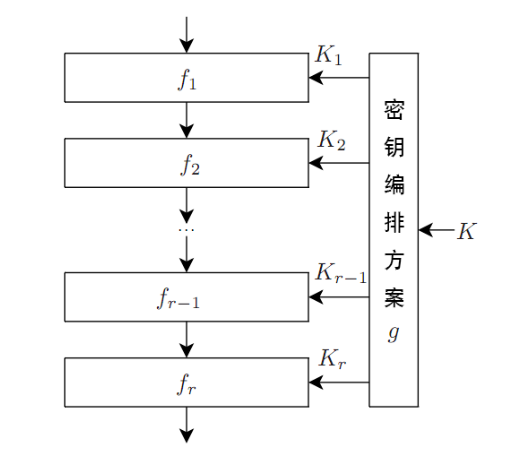
\includegraphics[width=5cm]{iterate}
    \bicaption[fig:Iterate]{迭代分组密码的一般结构}{迭代分组密码的结构}{Iterative Block Cipher}{The general structure}
\end{figure}
\begin{defn}[迭代分组密码]
    一个$r$轮的迭代分组密码$E$是一个$r$轮的带密钥置换的叠加,即:
    $$E(\cdot,k)=f_r(\cdot,k_r)\circ f_{r-1}(\cdot,k_{r-1})\circ\cdots\circ f_1(\cdot,k_1)$$
\end{defn}
其中$f_i(\cdot,k_i):\mathbb{F}^n_2\rightarrow\mathbb{F}^n_2$为第$i$轮轮函数,即依赖于轮密钥$k_i$的置换。
主密钥$K$经过密钥编排方案$g$生成$r$个轮密钥$RK_i$:
$$g:K\rightarrow(RK_1,RK_2,\dots,RK_r)$$

在一些迭代分组密码中,在第一轮轮函数开始前(或最后一轮结束后)会将明文(或密文)与一组子密钥进行异或,该组子密钥被成为白化密钥。
一般来说,为了软件和硬件上的实现效率,迭代分组密码的轮函数一般是相同的(部分密码在第一轮或最后一轮中会有些变化),因此在本文中我们会着重考虑分组密码的其中一轮的轮函数。
每一轮的轮函数一般包括三个部分:扩散层、非线性层和密钥引入层。
现有的迭代分组密码的整体结构基本可以分为以下三类:Feistel结构、SPN结构与Lai-Massey结构。除了上述三种主流结构外,整体结构还包括广义(非)平衡Feistel结构、MISTY结构以及各种结构的混合使用。

\section{高级加密标准AES}
为了取代DES,Rijndael在2000年被NIST选为高级加密标准(AES),它由Daemen和Rijmen共同设计\citen{daemen2013design}。AES具有128比特的分组长度,主密钥长度支持128比特、192比特和256比特(AES-128,AES-192和AES-256),所有操作面向字节(byte-oriented)。
其中,128比特密钥版本由10轮迭代,192比特迭代12轮,256比特迭代14轮。

在AES的轮函数中,每一轮的中间状态由一个$4\times 4$的矩阵表示,该状态矩阵中每一个位置对应一个字节。$K_r$为第$r$轮的轮密钥,同样由$4\times 4$的矩阵表示。
$X^{i,j}$表示矩阵(中间状态)$X$的第$i$行第$j$列的字节。
在第一轮加密开始前,明文$P_0$和白化密钥异或;最后一轮加密中,省略列混淆操作。每一轮加密的轮函数包含以下四个步骤:
\begin{enumerate}
    \item \textbf{字节代换(SubBytes)}:并行使用16个$8\times 8$的S盒;
    \item \textbf{行移位(ShiftRows)}:状态矩阵$X$的每一行循环移位相应字节数;
    \item \textbf{列混淆(MixColumns)}:状态矩阵的每一列都和矩阵$M_{MC}$相乘(见式\ref{eq:MC});
    \item \textbf{轮密钥加(AddRoundKey)}:状态矩阵每一字节和对应轮密钥矩阵的字节进行异或。
\end{enumerate}

AES的列混淆可以矩阵$M_{MC}$表示:
\begin{equation}
    M_{MC}=\left(
    \begin{array}{cccc}
        02&03&01&01\\
        01&02&03&01\\
        01&01&02&03\\
        03&01&01&02
    \end{array}
\right)
\label{eq:MC}
\end{equation}

列混淆是一个线性变换的过程。该变换使每一个输入字节都能影响同一列的四个输出的字节,同时一个输出字节也会依赖同一行的四个输入字节。
向量和矩阵的加法和乘法均在有限域$GF(2^8)$上完成,其中$GF(2^8)$上的加法为每比特逐位异或,$GF(2^8)$的乘法为模$P(x)=x^8+x^4+x^3+x+1$的乘法。
$M_{MC}$矩阵中的元素以16进制表示一个在$GF(2)$上的多项式,如“02”表示系数为00000010的多项式。
乘以“02”即为先将$x$左移1比特,再模余式$P(x)$。 

\section{分组密码的分析方法}
对任意一个分组密码,都存在如下4种攻击方法:穷尽密钥搜索、字典攻击、查表攻击和时间-空间权衡攻击。除了这4种通用的攻击方法,在对具体的分组密码算法进行安全性分析时,往往会针对其特殊的弱点产生其他的攻击方法。
对迭代分组密码而言,密码分析者首先将寻找一个简化轮数对应算法的有效区分器,然后通过猜测区分器之外的密钥来验证区分器的正确性。
下面给出常见的几种攻击方法:
\begin{enumerate}
    \item 由Biham和Shamir在1990年针对DES算法提出的差分密码分析\cite{biham1991differential},通过观察具有特定输入差分的明文对经过加密后的密文对的差分形式来恢复密钥;
    \item 由来学嘉教授给出的高阶差分分析\cite{lai1994higher}是一种采用了类似高阶导数概念的差分分析法,对差分函数再求差分;
    \item Matsui提出的线性密码分析\cite{matsui1993linear},如果密码算法的输入、输出比特的某个线性组合对应一个高概率偏差的线性表达式,就可以根据这个表达式来对密码算法进行恢复密钥攻击;
    \item Diffie和Hellman提出的中间相遇攻击\cite{diffie1977special},这是一种时间-空间权衡攻击方法,是不可能差分区分器的主要寻找方法之一,本文之后会提到一个对RECTANGLE的中间相遇攻击;
    \item Knudsen基于Daemen提出的Square攻击\cite{daemen1997block}而提出的更一般形式的积分攻击\cite{knudsen2002integral};
    \item Courtoi和Pieprzyk提出的代数攻击\cite{courtois2002cryptanalysis},通过求解一个多变元的代数方程来恢复密钥;
    \item Biham和Knudsen提出的相关密钥攻击\cite{biham1994new},该密码攻击更多地考虑了密钥编排方案的性质;
    \item 由Biryukov和Wagner提出的滑动攻击\cite{biryukov1999slide},对轮函数较弱、密钥编排方案又呈周期性的迭代分组密码较为有效。
\end{enumerate}

其中中间相遇攻击、相关密钥攻击和滑动攻击可以看做是针对密钥编排方案的攻击。这些攻击无一例外利用编排方案的弱点来获得更好的攻击效果,是目前为止利用密钥编排方案弱点最有效的两种攻击手段。

%# -*- coding: utf-8-unix -*-
%%==================================================
%% chapter01.tex for SJTU Master Thesis
%%==================================================

%\bibliographystyle{sjtu2}%[此处用于每章都生产参考文献]
\chapter{研究现状与本文概述}
\label{chap:Intro}
\section{研究现状}
密钥编排方案是在加密或是解密中都会用到的一种将较短的主密钥扩展成很长的扩展密钥(并用来做轮密钥)的算法。
在分组密码中,考虑到算法的设计与实现,其密钥编排方案往往会比较简单,而过于简单的编排方案往往会导致一些攻击。
在轻量级分组密码中,由于其不仅需要考虑安全性还需要考虑软硬件上的高效与简便的特殊性,这种情况更加普遍。
有些密钥编排方案是扩散程度较低的轮迭代算法,例如PRESENT\citen{Bogdanov},RECTANGLE\citen{zhang2015rectangle},TWINE\citen{Suzaki_2013}和LBlock\citen{Wu_2011};
有些密钥编排方案是简单的置换与线性操作,例如SIMON和SPECK\citen{beaulieusimon};
有些甚至根本没有编排方案,只是简单的在每轮中使用主密钥,例如LED\citen{Guo2011}。
这些密钥编排方案被高度简化,在实现上十分高效简便,但却导致了以相关密钥攻击\citen{biham1994new,Biryukov2009,Ko2004}和中间相遇攻击\citen{diffie1977special,Biryukov2015,Bogdanov2011}为主的攻击。

为了描述和量化密钥编排方案的扩散程度以及其导致攻击的具体的弱点所在,黄佳琳博士等人在\citen{huang2014revisiting}中提出了围绕“密钥信息”的一些概念,如计算路径、密钥依赖路径和实际密钥信息,这些概念形象生动地描述了一个密钥编排方案的扩散程度。
利用密钥编排方案中的密钥信息泄露,黄佳琳等人在\citen{huang2014revisiting}中提出了对40轮SHACAL-2密码\citen{Handschuh2002}和25轮XTEA密码\citen{Needham1997}的中间相遇攻击,并进一步在\citen{Huang_2014}中提出了一个能够给出一个编排方案的AKI合理上界的贪心算法。
然而,为了设计出一个能够在密钥信息上提供更好的安全性的密钥编排方案,我们需要AKI的精确值并从而总结出一个设计方案或原理。

\section{本文主要贡献}
在本文中,我们将会展示我们设计一种基于图论来解决AKI问题的多项式复杂度的算法,建立了密码学与图论之间的“桥梁”。
为了更完整的描述我们解决AKI问题的方法,我们将会从最简单的单轮AKI问题着手,并证明单轮编排方案与二分图的等价性;
之后我们将进一步介绍图论中著名的最大流最小割定理,并由此给出我们设计的AKI-最小割算法。
同时我们也对我们算法的正确性进行了理论证明。
通过计算出AKI的真正数值,我们成功地优化了针对23轮TWINE-80密码的零相关攻击,还设计了一种新的针对12轮RECTANGLE-128密码的中间相遇攻击。

同时,利用我们构建的密钥编排方案与流量网络之间的“桥梁”,我们也给出了一种能够构造出一种针对给定的子密钥集合没有信息泄露的,以依赖矩阵的形式表示的新的密钥编排方案的贪心算法。
基于这种算法,我们分别针对上述两个攻击,为TWINE-80设计了能够抵抗其零相关攻击的编排方案,也为RECTANGLE-128设计了能够抵抗所有8轮以上中间相遇攻击的新密钥编排方案。

关于上述算法的更多信息,请访问在\href{https://github.com/KirisameNanami/AKI-Algorithms}{Github}上的源码。

\section{本文结构安排}
本文的研究对象为分组密码的密钥编排方案,而研究贡献主要围绕AKI-最小割算法、单密钥集合的依赖矩阵设计算法及两者的应用。
本文的后续章节内容安排如下:

第三章为后续章节预备关于密钥信息的一系列概念与基本知识,并使用了黄佳琳在\citen{huang2014revisiting}中提出的玩具密码的例子来帮助理解;
并在黄佳琳对实际密钥信息(AKI)的定义上做略微扩展,使其应用范围更加普适,能够更广泛地应用在各种攻击中常见的密钥猜测集合中。

第四章中我们将介绍AKI-最小割算法来解决AKI问题。首先我们将AKI问题简化成仅有单轮加密情况下的子问题,描述并证明了该情况下密钥编排方案模型与二分图的等价性,并使用二分图最大匹配来解决这个子问题;
之后我们在介绍一个典型反例的帮助下,引出更加普遍情况下的AKI问题的解决方法。
我们将简单介绍图论中关于流量网络中流与割的定义,并介绍著名的最大流-最小割定理,为AKI-最小割算法的介绍与证明做准备;
随后我们将会介绍AKI-最小割算法的构图方法以及该流量网络与密钥编排方案之间的紧密关系;
为了证明AKI-最小割算法的正确性,我们使用最大流-最小割定理,从两个方向进行了证明,最终证明最小割与实际密钥信息集合的等价性。
最后,我们分析了AKI-最小割的时间复杂度,理论说明了该算法的高效性与实用性。

之后的第五章中,我们针对密钥信息泄露所导致的攻击列出了两个使用AKI-最小割算法的应用。
首先,我们对Wang和Lin等人提出的对23轮TWINE-80的两个零相关攻击进行了改正与优化,降低了猜测密钥集合的复杂度;
然后,我们提出了一个对12轮RECTANGLE-128的新的中间相遇攻击,由于这一类攻击可以十分简单的由AKI-最小割算法得出的结果得出,该攻击也侧面证明了密钥信息泄露的严重性。

在讨论了密钥信息泄露的攻击之后,我们转而在第六章中讨论如何设计密钥编排方案来防止密钥信息泄露。
在该章中我们将介绍一个对单个子密钥集合设计无密钥信息泄露的密钥编排方案的算法,利用最小费用最大流得出一个较小的密钥依赖矩阵;
使用该算法,我们对第五章中提到的TWINE的一个零相关区分器的密钥猜测部分进行了分析,并设计了一个新的密钥编排方案依赖矩阵使得该区分器的密钥猜测部分无法被优化,从而使该攻击的时间复杂度上升。
之后,我们介绍了如何为一个特定的轮函数设计无密钥信息泄露的密钥编排方案,并为一个特殊的例子——RECTANGLE-128设计了一个优化的密钥编排方案,
该密钥编排方案能够在理论上最少的轮数使AKI达到理论最大值,从而能够抵抗任意8轮以上的中间相遇攻击。

第七章中,我们将会介绍一系列相关工作,主要包含了使用AKI-最小割算法对各种不同分组密码算法的AKI分析。
首先,我们对两个十分相似的SPN结构轻量级分组密码PRESENT和RECTANGLE各自的两种密钥编排方案进行了分析,并对两者不同的结果的原因进行了讨论。
然后我们对两个拥有极其简单的密钥编排方案的密码算法Midori和LED进行了AKI分析,并将其与PRESENT和RECTANGLE相比较,讨论密钥编排方案与轮函数之间的紧密关系。
最后,在讨论了四种SPN结构密码函数后,为了说明Feistel结构的密码算法同样适用于我们的AKI-最小割算法,我们用SIMON这一经典的Feistel结构密码算法为例,详细说明了如何用AKI-最小割算法来分析Feistel结构密码函数,其中包含如何确定非简单迭代使用密钥扩展函数的密钥编排方案的依赖矩阵,以及Feistel结构密码的轮AKI的确定方法讨论。

%# -*- coding: utf-8-unix -*-
%%==================================================
%% chapter01.tex for SJTU Master Thesis
%%==================================================

%\bibliographystyle{sjtu2}%[此处用于每章都生产参考文献]
\chapter{AKI——实际密钥信息}
\label{chap:AKI}
轮函数的完全扩散性(completeness,即任意一个输出比特都依赖于所有的输入比特)是衡量一个轮函数扩散程度的重要标准。
对于非完全扩散的轮函数,考察其扩散的程度就变得极为重要。
为了精确考察密钥编排方案的弱点导致实际攻击的一般规律,黄佳琳博士在其博士毕业论文\citen{黄佳琳2014分组密码}中提出了实际密钥信息这一概念,从而考察了一个密钥编排方案在给定轮函数时的强弱程度。
\section{AKI的定义}
黄佳琳博士在\citen{huang2014revisiting}中提出了基于密钥依赖路径的实际密钥信息定义,而实际上实际密钥信息可适用于任何子密钥集合。因此,在本节中,我们扩展了黄佳琳博士对AKI的定义:
\begin{defn}[密钥信息集合]
    给定一个子密钥集合$K$,如果通过密钥编排方案,使用另一个子密钥集合$K_0$可以计算出$K$中的所有比特,则称$K_0$是$K$的一个密钥信息集合。
\end{defn}
\begin{defn}[实际密钥信息(AKI)]
    给定一个子密钥集合$K$,其密钥信息集合中最小的集合被成为实际密钥信息集合,实际密钥信息集合的大小即为$K$所包含的实际密钥信息。
\end{defn}
在实际密码攻击方法中,子密钥猜测环节十分常见且重要,例如相关密钥攻击\citen{biham1994new}和中间相遇攻击\citen{diffie1977special}.
在这些攻击中,将子密钥猜测集合替换为其实际密钥信息集合,就可以在不影响猜测的信息的情况下降低需要猜测的比特数量,从而降低攻击的复杂度。
\section{密钥编排方案的密钥信息}
黄佳琳博士在\citen{huang2014revisiting}中提出了使用AKI来分析给定一个轮函数的情况下一个密钥编排方案强弱的方法。
\begin{defn}[计算路径]
    设$O_0$为一个$m$比特的中间状态。根据轮函数我们可以得到一条$O_0$的计算路径:
    $$O_0=f_1(O_1,K_1)=f_1(f_2(O_2,K_2),K_1)=\dots f_1(\dots(f_s(O_s,K_s),K_{s-1}),\dots,K_1),$$
    其中$f_i$依赖于分组密码的结构和第$i$轮的轮函数,而$O_i$, $O_{i-1}$分别为第$i$轮的输入比特集合和输出比特集合。
    $O_0\rightarrow O_1\rightarrow O_2\rightarrow\dots\rightarrow O_s$被成为一条计算路径,其中$O_0$和$O_s$分别为该路径的输出和输入。
\end{defn}
为了构造$O_0$的一条计算路径,我们需要从$O_0$开始往前轮寻找所有计算$O_0$所需要的比特,而这些比特加上$O_0$本身则构成了$O_0$的一条计算路径。
\begin{defn}[密钥依赖路径]
    一条计算路径上所涉及的所有轮密钥比特所构成的集合称为该计算路径的密钥依赖路径。
\end{defn}
密钥依赖路径实际上包含了为了计算$O_0$所需要的所有的轮密钥比特。

一般来说,一个密钥编排方案包含了密钥提取和密钥扩展两个部分。
\begin{defn}[密钥提取]
    密钥提取是密钥编排方案中从第$i$轮的密钥寄存器中的子密钥$WK_i$提取出要使用在轮函数中的轮密钥$RK_i$的过程。
\end{defn}
\begin{defn}[密钥扩展]
    密钥提取是密钥编排方案中从第$i$轮的密钥寄存器中的子密钥$WK_i$生成第$i+1$轮的子密钥$WK_{i+1}$的过程。
\end{defn}
由于对于一个密钥编排方案来说,改变密钥提取方案本质上只是改变了子密钥$WK_i$中比特的顺序,因此为了将目光着重放在密钥扩展上,
在本文中,凡是未提前定义的密钥编排方案,其密钥提取方案默认为简单提取,即$RK_i^j=WK_i^j$。
当密钥提取均为简单提取时,密钥依赖路径的计算就只依赖于轮函数,与密钥编排方案无关,因此给定轮函数的情况下,不同密钥编排方案下同一条密钥依赖路径的实际密钥信息的不同可以用来考察该密钥编排方案在此轮函数情况下的强弱程度。

接下来,我们给出对于一个加密方案,单轮的AKI的定义:
\begin{defn}[单轮实际密钥信息]
    一个加密方案中,第$i$轮的单轮实际密钥信息是该轮中间状态$X_i$中所有单个比特对应的密钥依赖路径的实际密钥信息的最小值。
    \label{def:RoundAKI}
\end{defn}
单轮实际密钥信息描述了该轮所包含的密钥信息的下界。
对于衡量一个密钥编排方案来说,这是一个重要的指标。
我们会在第\ref{chap:App}、\ref{chap:Design}和\ref{chap:Work}章中多次使用这个定义。
为了更方便的计算以上两条路径,我们需要量化轮函数和密钥编排方案中输入比特和输出比特的依赖关系。
\begin{defn}[依赖矩阵]
    一个依赖矩阵$M=M_{i,j}\in\mathbb{F}^{n\times n}_2$包含了单轮输入输出比特之间的依赖关系,其中$M_{i,j}=1$表示第$i$个输出比特依赖于第$j$个输入比特,反之$M_{i,j}=0$表示不依赖。\footnote{值得一提的是,加密算法和解密算法所对应的依赖矩阵不一定互为逆矩阵,需要以实际情况推论。}
\end{defn}
\begin{figure}[htbp]
\centering
    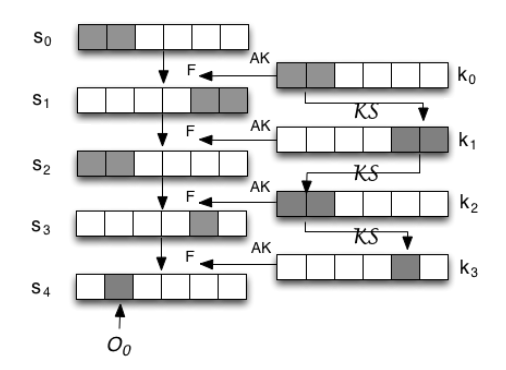
\includegraphics[width=6cm]{ToyCipher}
    \bicaption[fig:toy]{玩具密码}{一个4轮的玩具密码}{ToyCipher}{A 4-round toy cipher}
\end{figure}
\textbf{一个典型的例子\citen{Huang_2014}:}
图\ref{fig:toy}是一个4轮SPN结构的玩具密码,其分组大小和主密钥长度均为6比特,每一个中间状态都直接与相对应的轮密钥进行异或。
其轮函数依赖矩阵为$M_s$,密钥编排方案的依赖矩阵为$M_k$(这里给出了三个不同的编排方案$M_{k1},M_{k2},M_{k3}$)。
$$M_s=\left(
    \begin{array}{cccccc}
        0&0&0&0&0&1\\
        0&0&0&0&1&1\\
        0&0&0&1&0&0\\
        0&0&1&1&0&0\\
        0&1&0&0&0&0\\
        1&1&0&0&0&0
    \end{array}
\right)$$
$$M_k=\left(
    \begin{array}{cccccc}
        0&0&0&0&0&1\\
        0&0&0&0&1&1\\
        0&0&0&1&0&0\\
        0&0&1&1&0&0\\
        0&1&0&0&0&0\\
        1&1&0&0&0&0
    \end{array}
\right)
or\left(
    \begin{array}{cccccc}
        1&0&0&0&0&0\\
        0&1&0&1&0&0\\
        0&0&0&0&1&0\\
        1&0&0&0&0&1\\
        0&0&1&0&0&0\\
        0&0&0&1&0&1
    \end{array}
\right)
or\left(
    \begin{array}{cccccc}
        1&0&1&0&0&0\\
        0&0&0&1&0&0\\
        0&1&0&0&1&0\\
        1&0&0&0&0&0\\
        0&0&1&0&0&1\\
        0&0&0&0&1&0
    \end{array}
\right)$$
令$O_0$只保含了第4轮的第2比特(记为$X_4^1$),我们可以根据轮函数依赖矩阵$M_s$计算出其计算路径:$\{X_0^0,X_0^1\}\rightarrow \{X_1^4,X_1^5\}\rightarrow \{X_2^0,X_2^1\}\rightarrow \{X_3^4\}\rightarrow \{X_4^1\}$。
相对应的,其密钥依赖路径为$\{WK_0^0,WK_0^1\}\rightarrow \{WK_1^4,WK_1^5\}\rightarrow \{WK_2^0,WK_2^1\}\rightarrow \{WK_3^4\}$。
注意到密钥依赖路径中包含了7比特的子密钥,但考虑到主密钥长度只有6比特,因此该密钥依赖路径的所包含的实际密钥信息理论上不可能超过6比特。

在三个密钥编排方案中,密钥编排方案$M_{k1}$由于其与轮函数的依赖关系完全一样,导致密钥依赖路径上各轮比特之间存在与轮函数完全一致的依赖关系,则只用密钥依赖路径在主密钥上的比特就可以推出整条密钥依赖路径。
因此,$\{WK_0^0,WK_0^1\}$就是该密钥依赖路径的一个实际密钥信息集合,AKI仅为2,存在着严重的密钥信息泄露。

而相对的,密钥编排方案$M_{k2}$和$M_{k3}$就表现更好。在编排方案$M_{k2}$下,该密钥依赖路径的AKI为5(其中一个可能的实际密钥信息集合为$\{WK_0^0,WK_0^1,WK_0^2,WK_0^3,WK_0^5\}$),而$M_{k3}$更让AKI达到了理论最大值6。
值得一提的是,$M_{k3}$能够使所有第4轮比特的密钥依赖路径的AKI都达到理论最大值6,即$M_{k3}$使得该玩具密码在经过4轮加密之后不存在任何密钥信息泄露。

因此,AKI不仅在攻击中能够降低某些攻击的复杂度,并且一个密钥编排方案的AKI值也是在某种程度上衡量该方案在其轮函数下的强弱程度的重要参数,而后者中的弱编排方案将会导致该密码函数更容易受到前者的影响,降低攻击该函数的复杂度。
同时,由于给定轮函数后不同的编排方案拥有不同的AKI值,使得AKI成为了设计与优化密钥编排方案的重要指标。

%# -*- coding: utf-8-unix -*-
%%==================================================
%% chapter01.tex for SJTU Master Thesis
%%==================================================

%\bibliographystyle{sjtu2}%[此处用于每章都生产参考文献]
\chapter{AKI算法}
\label{chap:Alg}

为了确定一个子密钥集合$K$的实际密钥信息,我们需要一个算法来计算AKI的值并得到一些可能的实际密钥信息集合。
黄佳琳博士在其博士论文\cite{huang2014revisiting}中提出了一个自动化搜索密钥信息泄露的工具,但该工具设计的算法是一个贪心算法,只能计算出AKI的一个合理上界,无法得到真实的AKI值。
一个AKI的合理上界可以用来进行攻击可能性的分析,但无法用来实际分析一个密钥编排方案的强弱。
Lin等人在\citen{lin2016automatic}中提出了一种对密钥桥技术(Key-Bridging Technique\citen{dunkelman2010improved})的自动化搜索算法,但时间复杂度极高,无法进行大量不同$K$的计算,并且也存在一些反例无法计算(后文中将会提到一个反例)。
因此,现有的AKI算法由于只能给出AKI的一个合理上界,只能用于攻击分析,无法用来分析密钥编排方案的强弱好坏,也不能用来改进密钥编排方案的设计。
本章将会介绍一种全新的基于图论的AKI算法,将会在多项式时间复杂度内计算出真实的AKI值。

\section{单轮加密的AKI}
在介绍完整的AKI算法之前,我们首先从简化版的问题开始考虑——仅有一轮加密时的AKI计算。
我们假设子密钥集合$K$全部集中在第$r$轮上,然后只考虑$r$轮和$r-1$轮两轮之间的依赖关系。
为了解决这个问题,我们将使用图论中二分图的思想来将编排方案、密钥比特、依赖关系等参数量化成图,进而将AKI的计算转化为一个图论的问题。
\begin{defn}[二分图]
    设$G(V,E)$是一个无向图,如果顶点集合$V$可以分割为两个互不相交的子集$A,B$且图中每条边的两个顶点分别属于不同的子集,则称$G$为一个二分图,可记为$G(A,B,E)$。
\end{defn}
\begin{figure}
    \centering
    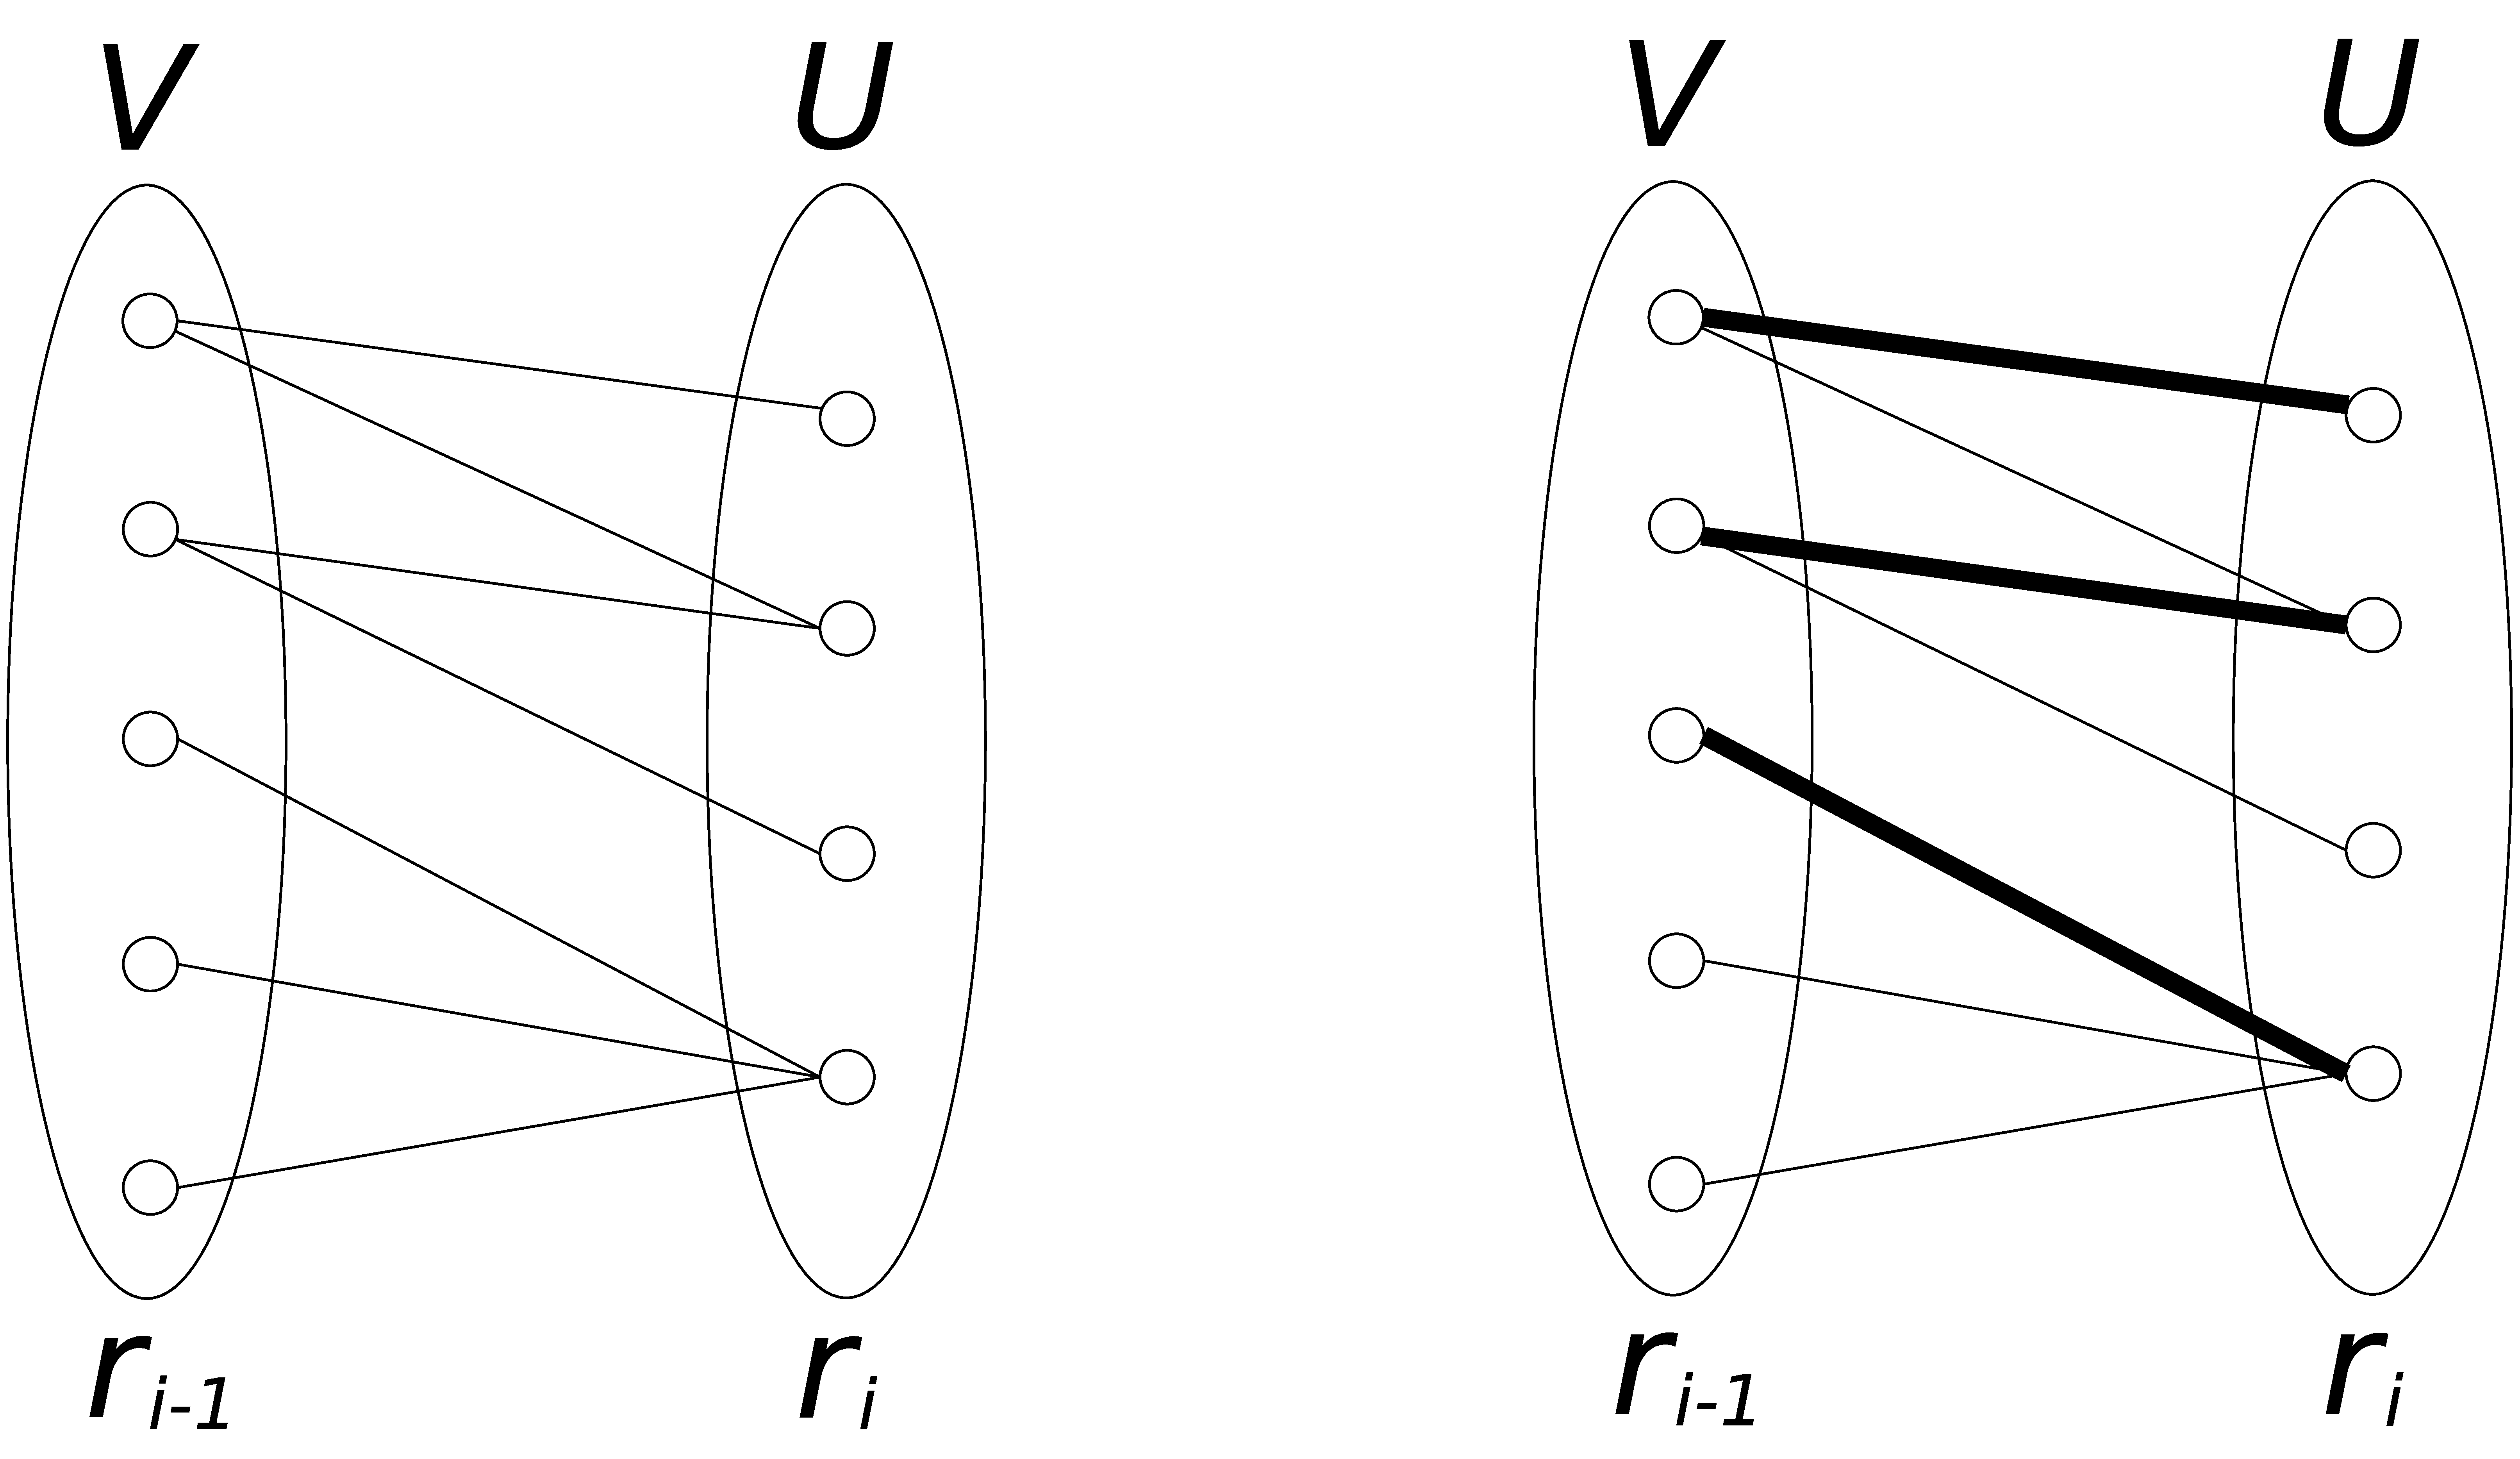
\includegraphics[height=4cm]{bipartite}
    \bicaption[fig:bigraph]{二分图}{一个二分图的例子和它其中一中匹配(被加粗的边)}{Bipartite Graph}{An example of bipartite graph and one of its matching (bold edges)}
\end{figure}
\begin{defn}[图的匹配]
    设$G(V,E)$是一个无向图,如果一个边集$M\subseteq E$中的边两两不相邻(即任意两条边不存在公共的顶点),则成$M$是$G$的一个匹配。
\end{defn}
图\ref{fig:bigraph}中的例子$G(U,V,E)$是一个典型的二分图。我们可以看到所有的边都横跨在两个点集$U,V$之间,而点集的内部不存在任何的边。
在二分图理论中最著名的问题莫过于“二分图最大匹配”问题\citen{west2001introduction},其旨在二分图$G(U,V,E)$中寻找一个最大的匹配$M$。
为了计算最大匹配的值$|M|$,我们需要引入组合数学中著名的霍尔定理\citen{hall1935representatives}的一个拓展:
\begin{thm}[霍尔定理\cite{hall1935representatives}的一个拓展]
    在一个二分图$G(U,V,E)$中,取$U$中的一个子集$X\subseteq U$,记$\Gamma(X)$为$X$的“邻居”,即所有$V$中与$X$中点相邻的点的集合。
    令$\delta(U)=max_{X\subseteq U}\{|X|-|\Gamma(X)|\}$,则有:
    $$MaxMatching(G)=|U|-\delta(U)$$
    \label{thm:hall}
\end{thm}
为了建立轮AKI问题与二分图之间的关系,我们需要这样思考:$r-1$轮和$r$轮的子密钥分别对应子集$V$和$U$中的一个顶点,而这两轮比特之间的一条依赖关系对应横跨$U,V$之间的一条边。
对于给定的子密钥集合$K$(均在$r$轮上),我们把$K$中所有的比特转化成顶点集合$U$,将$K$所依赖的所有$r-1$轮的比特转化为顶点集合$V$,他们之间的依赖关系转化为边集$E$,这样就可以构造出一张二分图$G(U,V,E)$。
这样构造之后,我们重新考虑定理\ref{thm:hall}中的子集$X$(可以视为$K$的一个子比特集合),它的“邻居”$\Gamma(X)$实际上包含了$X$依赖的所有$r-1$轮上的比特,即用$\Gamma(X)$中的所有比特可以推出$X$中的所有比特。
因此,我们可以得出以下引理:
\begin{lem}
    给定一个集中在一轮上的子密钥集合$K$和它的一个子集$X$,令$K'=\Gamma(X)\cup(K\backslash X)$,则$K'$是$K$的一个密钥信息集合。
\end{lem}
\begin{proof}
    由于$\Gamma(X)$可以推出$X$,而$K\backslash X$显然可以推出$K\backslash X$本身,则$K'$可以推出$K$,因此$K'$是$K$的一个密钥信息集合。
\end{proof}
为了找出$K$的实际密钥信息集合,我们需要找到一个最小的密钥信息集合。由于
$$|K'|=|K|-|X|+|\Gamma(X)|=|K|-(|X|-|\Gamma(X)|)$$
又由前文构造出的图$G(U,V,E)$,我们可以得到实际密钥信息集合$K'_{min}$必然满足:
\[
\begin{split}
    |K'_{min}|&=min\{|K|-|X|+|\Gamma(X)|\}\\
              &=|U|-max_{X\subseteq U}\{|X|-|\Gamma(X)|\}\\
              &=|U|-\delta(U)=MaxMatching(G) \qquad\ref{thm:hall}
\end{split}
\]
因此,一个子密钥集合$K$的实际密钥信息的值等于由$U=K$构造出的二分图$G(U,V,E)$的最大匹配的值,且实际密钥信息集合为$K'_{min}=\Gamma(X_{max})\cup(K\backslash X_{max})$,其中$X_{max}$是使$|X|-|\Gamma(X)|$最大的$X$。

\section{AKI-最小割算法}
aaaaa

%# -*- coding: utf-8-unix -*-
%%==================================================
%% chapter01.tex for SJTU Master Thesis
%%==================================================

%\bibliographystyle{sjtu2}%[此处用于每章都生产参考文献]
\chapter{密钥信息泄露的应用}
\label{chap:App}
由于实际密钥信息集合中包含了和给定的子密钥集合$K$相同大小的密钥信息,因此只要其中存在密钥信息泄露,基于猜测集合$K$的攻击(这些攻击中$K$一般用来猜测一个区分器的输入/输出)就可以通过用$K$的实际密钥信息集合$K'_0$代替$K$成为猜测集合来降低其复杂度。
在本章中,我们将会介绍两种基于密钥信息泄露的AKI的应用。

\section{对TWINE-80的零相关攻击}
Yanfeng Wang等人在\citen{wang2014improved}中通过其提出的$((2,9),4,14,5)$这一区分器给出了一个对23轮TWINE-80密码的多维零相关线性攻击,而Li Lin等人在\citen{lin2016automatic}中指出了Wang在其文章中错误使用的密钥桥,并给出了一个基于区分器$((6,9),4,14,5)$的新的23轮攻击,并给出了3个密钥桥来降低其复杂度。
然而,Lin提出的密钥桥中,$RK^6_{22}\oplus S(RK^2_{22})\oplus S(RK^5_{22})\Rightarrow RK^6_2$并不能用来降低他们提出的23轮攻击,因为$RK^6_2$并不在$X^6_4$的密钥依赖路径中。
我们使用我们的AKI-最小割算法,重新分析了上述两个攻击,发现他们都可以由原来的19个密钥块组成的猜测集合降低为一个16个密钥块组成的实际密钥信息集合。
表\ref{tab:twine}展示了两种攻击的猜测集合和实际密钥信息集合。
\begin{table}[htbp]
    \centering
    \begin{tabular}{c|c|c}
        区分器 & 猜测集合 & 实际密钥信息集合\\
        \hline
        \multirow{4}{*}{((2,9),4,14,5)} & $WK^3_0|WK^4_0|WK^6_0|WK^{13}_1|WK^{15}_1$ & $WK_0^0|WK_0^3|WK_0^4|WK_0^6|WK_0^{14}$\\
                                        & $WK^6_2|WK_3^{13}|WK_{18}^{13}|WK_{19}^{15}|WK_{20}^3$ & $WK_0^{15}|WK_0^{17}|WK_0^{18}|WK_0^{19}$ \\
                                        & $WK_{20}^{16}|WK_{21}^1|WK_{21}^{13}|WK_{21}^{14}|WK_{22}^4$ & $WK^0_6|WK^0_9|WK_{10}^0$\\ 
                                        & $WK_{22}^6|WK_{22}^{13}|WK_{22}^{14}|WK_{22}^{15}$ & $WK_{13}^0|WK_{13}^{16}|WK_{19}^{16}|WK_{20}^{16}$ \\
        \hline
        \multirow{4}{*}{((6,9),4,14,5)} & $WK^3_0|WK^6_0|WK^{16}_0|WK^4_1|WK^{16}_1$ & $WK_0^0|WK_0^1|WK_0^3|WK_0^6|WK_0^7$\\
                                        & $WK^{15}_2|WK_3^{14}|WK_{18}^{13}|WK_{19}^{15}|WK_{20}^3$ & $WK_0^8|WK_0^{15}|WK_0^{16}|WK_0^{18}$ \\
                                        & $WK_{20}^{16}|WK_{21}^1|WK_{21}^{13}|WK_{21}^{14}|WK_{22}^4$ & $WK^0_6|WK_6^{16}|WK_9^0$\\ 
                                        & $WK_{22}^6|WK_{22}^{13}|WK_{22}^{14}|WK_{22}^{15}$ & $WK_{9}^{16}|WK_{13}^{16}|WK_{19}^{16}|WK_{20}^{16}$ \\
        \hline
    \end{tabular}
    \bicaption[tab:twine]{对TWINE-80的攻击的优化}{两种区分器下的19密钥块的猜测集合和16密钥块的实际密钥信息集合}{Optimization for attacks on TWINE-80}{The 19-nibble subkey set and 16-nibble AKI-set of two different distinguishers of TWINE-80}
\end{table}

\section{对RECTANGLE-128的中间相遇攻击}
本节中我们将会结合基础的中间相遇技术和RECTANGLE的密钥弱点来得出一个对RECTANGLE-128的12轮中间相遇攻击。
我们的攻击的数据复杂度只有8个已知明文,时间复杂度为$2^{126.32}$次加密,空间复杂度低于$2^{125}$个128比特分组。
在接下来的讨论中,我们认为12轮简化的RECTANGLE拥有12轮的加密方程和一个最终的白化密钥加步骤。

我们设定中间相遇的中间值$V$为第6轮中的4比特密文$X_6^0,X_6^4,X_6^8,X_6^{12}$,其计算可以分为加密和解密两种方法。
在加密方向上,计算$V$可以使用明文$X_0$和子密钥集合$K_t$;而在解密方向上,计算$V$需要用到密文$X_{12}$和子密钥集合$K_b$。

在加密方向上,6轮向前的计算路径的密钥依赖路径上共计由288比特的轮密钥,而在解密方向的6轮向后计算路径的密钥依赖路径上共计由292比特的轮密钥,即$|K_t|=288$,$|K_b|=292$。
也就是说,为了计算$X_6^0,X_6^4,X_6^8,X_6^{12}$,我们需要在前6轮加密中猜测288比特密钥,在后6轮解密中猜测292比特密钥,而这样做的代价是无法形成一个攻击的。
然而,无论是向前的路径还是向后的路径,由于RECTANGLE-128密钥编排方案的信息泄露,两者的AKI均只有124,也就是说只要124比特的子密钥就足以得出所有$K_t$或是$K_b$中所有的子密钥比特了,这样就使得12轮的中间相遇攻击变为可能。
图\ref{fig:12}展示了该攻击的计算路径和密钥依赖路径$K_t$和$K_b$,其实际密钥信息集合分别陈列在附录\ref{AppendixA}中。为了方便描述,我们记$K'_t$为$K_t$的实际密钥信息集合,相对应的$K'_b$为$K_b$的实际密钥信息集合。
\begin{figure}
\centering
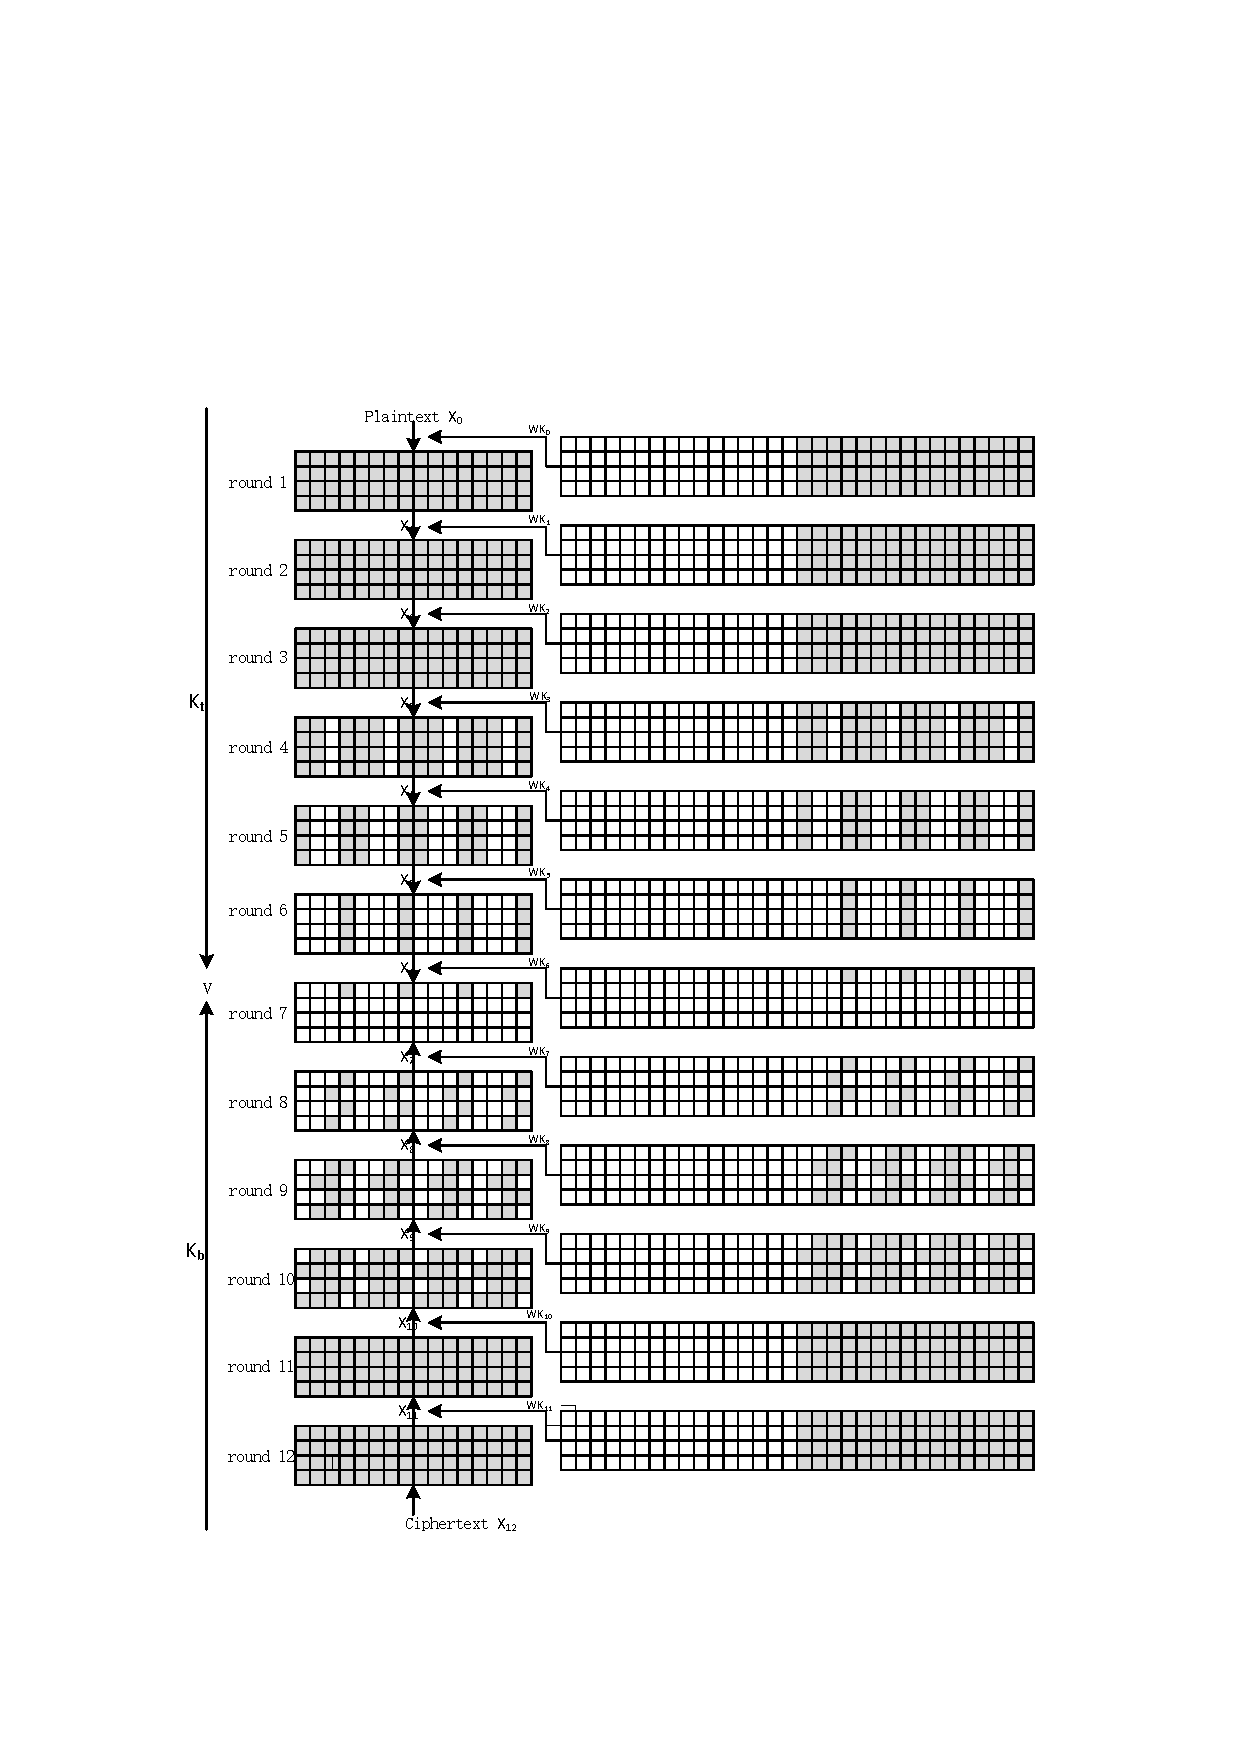
\includegraphics[width=130mm]{12.pdf}
\bicaption[fig:12]{对RECTANGLE-128的12轮中间相遇攻击}{一条6轮的前向(后向)计算路径(左)和密钥依赖路径(右)}{12-round MITM attack}{A 6-round forward (backward) Computation Path (left) and the Key Dependency Path (right).}
\end{figure}
 
在我们的攻击中,每次猜测$K'_t$(从而推出$K_t$),我们计算出相对应的$V$并将其存在一个哈希表中。
同样,每次猜测$K'_b$,计算出相应的$V$并在哈希表中寻找与他匹配的$K_t$。
如果在两个方向上的计算的出了相同的$V$,那么哈希表中将会由这样一对匹配,这个匹配所对应的密钥猜测$(K_t,K_b)$就会被认为是一个候选的密钥猜测。
算法\ref{alg:MITM}中包含了该攻击的伪代码。
\begin{algorithm}
\footnotesize
\caption{对RECTANGLE-128的12轮中间相遇攻击}
\label{alg:MITM}
\begin{algorithmic}[1]
\For {所有可能的124比特$K^{\prime}_t$的值}
\State 推测出$K_t$中的比特;
\State 将明文$P_i$加密以得到$X_6^0[i],X_6^4[i],X_6^8[i],X_6^{12}[i]$, $i=1,\dots,8$;
\State 将$K^{\prime}_t$存储到哈希表$T_1$,目录为$X_6^0[1],X_6^4[1],X_6^8[1],X_6^{12}[1]||\dots||X_6^0[8],X_6^4[8],X_6^8[8],X_6^{12}[8]$;
\EndFor
\For {所有可能的124比特$K^{\prime}_b$的值}
\State 推测出$K_b$中的比特;
\State 将明文$C_i$加密以得到$X_6^0[i],X_6^4[i],X_6^8[i],X_6^{12}[i]$, $i=1,\dots,9$;
\If {以$X_6^0[1],X_6^4[1],X_6^8[1],X_6^{12}[1]||\dots||X_6^0[8],X_6^4[8],X_6^8[8],X_6^{12}[8]$为目录的数据存在于哈希表$T_1$中}
\State 取出相对应的$K^{\prime}_t$和现有的$K^{\prime}_b$组成一个候选的蜜月猜测.
\EndIf
\EndFor
\State 枚举得到的所有的候选密钥.
\end{algorithmic}
\end{algorithm}

根据密钥编排方案,在猜测出所有$K'_t$的124比特后,$K'_b$中由92比特也可以被推出。
因此,这两条密钥依赖路径共享了92比特的密钥信息,我们就可以分离出这92比特来减少穷搜的时间复杂度。

\noindent
\textbf{复杂度分析:}在该12轮攻击中,我们使用了8个已知明密文对。攻击的时间复杂度为$\mathcal{O}(2^{124})$。
更精确的来说,在中间相遇部分共有$2^{124\cdot 8\cdot 0.5}=2^{126}$次12轮加密,剩下的候选密钥共有$2^{124+124-92-4\cdot 8}=2^{124}$个。
因此,在枚举阶段需要$2^{124}$个完整的加密。总共的时间复杂度为$2^{126.32}$次12轮RECTANGLE-128的加密过程。
空间复杂度为$\mathcal{O}(2^{124})$。更精确的来说,我们需要$2^{124}$个大小为$4\cdot 8+124=156$比特的分组,小于$2^{125}$个128比特的分组。

我们的攻击是第一个对RECTANGLE-128的拥有非常低数据复杂度的攻击。
实际上,在\citen{bouillaguet2011automatic}中也提到,为了更好的安全性理解,确定仅用非常少的可用数据最多可以攻击多少轮非常重要。
尽管这个攻击可能不是针对RECTANGLE-128最好的攻击,但是类似这种的中间相遇攻击可以非常容易地由其密钥编排方案的信息泄露得出,而这在某种程度上体现了密钥信息泄露的严重后果和AKI的重要性。

%# -*- coding: utf-8-unix -*-
%%==================================================
%% chapter01.tex for SJTU Master Thesis
%%==================================================

%\bibliographystyle{sjtu2}%[此处用于每章都生产参考文献]
\chapter{密钥编排方案的设计}
\label{chap:Design}
在前几章的讨论中,我们将密钥编排方案通过算法\ref{alg:const}量化成了一个流量网络。
在此基础上,我们可以进一步考虑如何去设计一个密钥编排方案,让它在密钥信息这一方面上表现得更好。
理论上,对于一个主密钥长度为$n$的密码函数,给定一个子密钥集合$K$,如果$|K|\geq n$,则必然存在一个密钥编排方案能够让$K$的AKI达到$n$。
这个结论在密钥编排方案完全扩散(即其依赖矩阵为全1矩阵)时十分显而易见,但是全扩散的密钥编排方案并不能在实际中得到运用。
因此,我们需要一个尽可能小的(1的数量尽可能少的)依赖矩阵来达到实际运用的目的。

\section{单个子密钥集合下的矩阵设计}
给定一个子密钥集合$K$,设计一个尽可能小的依赖矩阵$M$使得集合$K$的AKI达到$n$。
子密钥集合猜测的技术在许多攻击中都有设计,我们在第\ref{chap:App}章中讨论了两种设计密钥猜测的攻击方式。
在这一节中,我们将给出一个贪心算法来输出一个相对较小的矩阵$M$。

简单来说,在我们的贪心算法算法\ref{alg:Matrix}中,我们在由$K$和全1矩阵$M_{full}$通过算法\ref{alg:const}所建立起来的流量网络$G_f$的基础上,给每一条弧都新添加一个参数$cost$表示费用。
除了像$(u_{out},v_{in})$这样的代表前后轮比特依赖关系的弧的费用是1以外,别的所有弧的费用均为0.
然后,我们计算出流量网络$G_f$的一个最小费用最大流\footnote{最小费用最大流值的是在有费用的流量网络$G_f$中所有最大流中费用最小的流,其中流的费用被定义为$\sum f(e)\cdot cost(e)$}后,将该流中所有涉及到的弧提取出来形成一个新的矩阵$M$(可以看成将所有弧压缩到一轮中)。
由于$G_f$是由全扩散的密钥编排方案构造出来的,我们计算出的最小费用最大流$f$的流量显然是$n$;
又注意到如果我们重新由$K$和$M$构造出一个新的流量网络$G'_f$,上述的最小费用最大流$f$在该网络中依然成立,因为所有$f$涉及的弧都被存在了$M$中。
因此,该矩阵$M$将会使$K$的AKI为$n$。
同时,由于我们对该流“费用最低”的要求,$f$保证了涉及尽可能少的依赖关系(但没有考虑在不同轮中共用同一种依赖关系的可能性),因此$M$将会是一个符合条件的相对较小的矩阵(但不一定是最小的)。
\begin{algorithm}
    \caption{矩阵设计算法}
    \begin{algorithmic}[1]
        \Function{GetMatrix}{$K$}
            \State $G \gets$\Call{Construct}{$K,M_{full}$}
            \ForAll{$e\in G.E$}
            \State $cost(e)\gets 0$
            \EndFor
            \ForAll{$(u_{out},v_{in})\in G.E$}
            \State $cost((u_{out},v_{in}))\gets 1$
            \EndFor
            \State $f \gets$\Call{Get\_Min\_Cost\_Max\_Flow}{$G(E,V,c),cost$}
            \State $M \gets \mathbf{0}$
            \ForAll {$f((u_{out},v_{in}))>0$}
            \State $M[u.bit][v.bit]\gets 1$
            \EndFor
            \State \Return $M$
        \EndFunction
    \end{algorithmic}
    \label{alg:Matrix}
\end{algorithm}

注意到$M$可以是密钥编排方案的一个中间矩阵,也就是说你可以为了更方便的以$M$为基础设计编排方案,在$M$中添加额外的1且保持AKI为$n$。

\noindent
\textbf{应用于对TWINE-80的攻击:}我们在第\ref{chap:App}章中提到了一个使用$((2,9),4,14,5)$区分器的对TWINE-80的23轮零相关攻击。
在这个攻击中,我们使用了TWINE-80密钥编排方案的密钥信息泄露,将原本由19密钥块大小的猜测子密钥集合$K$降低到了16子密钥块的大小。
为了让这个优化变得不可能,我们需要重新设计一个密钥编排方案来让$K$的AKI达到理论上最大(19个子密钥块)。
由算法\ref{alg:Matrix},我们找到了如下矩阵:
$$\left(
    \begin{array}{cccccccccccccccccccc}
0&0&0&0&0&0&0&0&0&0&0&0&0&0&0&0&0&0&0&0\\
0&0&0&0&0&0&0&0&0&0&0&0&0&0&0&0&0&1&0&0\\
0&0&0&0&0&0&0&0&0&0&0&0&0&0&0&0&0&0&0&0\\
0&0&0&0&0&0&0&0&0&0&0&0&0&0&0&0&0&0&1&0\\
0&1&0&0&0&0&0&0&0&0&0&0&0&0&0&1&0&0&0&0\\
0&0&1&0&0&0&0&0&0&0&0&0&0&0&0&0&0&0&0&0\\
0&0&0&0&0&1&0&0&0&0&0&0&0&0&0&0&1&0&0&1\\
0&0&0&0&1&0&0&1&0&0&0&0&0&0&0&0&0&0&0&0\\
0&0&0&0&0&1&0&1&1&0&0&0&0&0&0&0&0&0&0&0\\
0&0&0&0&0&0&1&0&1&1&0&0&0&0&0&0&0&0&0&0\\
0&0&0&0&0&0&0&1&0&1&1&0&0&0&0&0&0&0&0&0\\
0&0&0&0&0&0&0&0&1&1&1&1&0&0&0&0&0&0&0&0\\
0&0&0&0&0&0&0&0&0&1&1&1&1&0&0&0&0&0&0&0\\
0&0&0&0&0&0&0&0&0&0&1&1&1&1&0&0&0&1&1&1\\
0&0&0&0&0&0&0&0&0&0&0&1&1&1&1&0&0&0&1&1\\
0&0&0&0&0&0&0&0&0&0&0&1&1&1&1&1&0&0&0&1\\
0&0&0&0&0&0&0&0&0&0&0&0&1&0&1&1&1&0&0&1\\
0&0&0&0&0&0&0&0&0&0&0&0&0&1&1&1&1&1&0&0\\
0&0&0&0&0&0&0&0&0&0&0&0&0&0&1&0&1&1&1&0\\
0&0&0&0&0&0&0&0&0&0&0&0&0&0&0&1&0&1&1&1\\
\end{array}
\right)
$$

\section{为轮函数设计密钥编排方案}
黄佳琳博士在\citen{huang2014revisiting}提出了利用AKI来评估密码算法的密钥编排方案的方法,即分析一轮中所有比特的密钥依赖路径的实际密钥信息,进而用该轮最低的AKI来确定密钥编排方案经过该轮次后是否存在密钥信息泄露。
理论上,一旦密钥依赖路径的大小超过了主密钥长度$n$,该轮的实际密钥信息就可能能够达到$n$。
注意到密钥依赖路径的大小只与计算路径有关,而计算路径只依赖于轮函数,因此在给定轮函数的情况下,我们就可以确定从哪一轮开始实际密钥信息能够在理论上达到最大值$n$。
因此,寻找一个理想的密钥编排方案就相当于寻找一个尽可能小的依赖矩阵$M$使得第$r_0$轮(该轮的密钥依赖路径大小开始超过$n$)的实际密钥信息达到$n$。
但由于一整轮的实际密钥信息是该轮所有密钥依赖路径的实际密钥信息的最小值,要寻找一个矩阵$M$使得所有密钥依赖路径$K_1,K_2,\dots$的AKI都达到$n$是一个十分困难的问题,我们暂时无法想到一个有效的计算方法。
但我们仍然相信我们构建出的密钥编排方案与流量网络的“桥梁”将会帮助我们找到密钥编排方案的设计原则。

\section{一个RECTANGLE-128的优化密钥编排方案}
我们计算了RECTANGLE-128的实际密钥信息,找到了它的密钥编排方案存在着比较严重的密钥信息泄露。
这个泄露所导致的中间相遇攻击在第\ref{chap:App}章中已有所讨论。表\ref{tab:Rec}中展示了其具体的AKI值。
\begin{table}[htbp]
    \centering
    \begin{tabular}{c|c|c|c|c}
        \multirow{2}{*}{轮数} & \multicolumn{2}{c|}{RECTANGLE-128} & 简单移位方案 & 优化后的编排方案\\
        \cline{2-5}
        & 理论值 & $|AKI|$ & $|AKI|$ &$ |AKI| $\\
        \hline
        $r=1$ & 4 & 4 & 4 & 4\\
        $r=2$ & 20 & 18 & 20 & 20\\
        $r=3$ & 56 & 44 & 52 & 53\\ 
        $r=4$ & 120 & 83 & 100 & 102\\ 
        $r=5$ & 128 & 103 & \textbf{128} &\textbf{128}\\ 
        $r=6$ & 128 & 120 & 128 & 128\\ 
        $r=7$ & 128 & \textbf{128} & 128& 128\\ 
        \hline
    \end{tabular}
    \bicaption[tab:Rec]{RECTANGLE-128在不同密钥编排方案下的实际密钥信息}{RECTANGLE-128在其原编排方案、简单移位方案和优化方案下的实际密钥信息}{AKI of RECTANGLE-128}{The AKI of the RECTANGLE-128 schedule and the optimized schedule}
\end{table}
\begin{algorithm}
    \caption{RECTANGLE-128原密钥编排方案的密钥扩展函数}
    \begin{algorithmic}[1]
        \Function{OriginalScheduleFunc}{$WK_{i-1}$}
        \State $WK_i \gets$ \Call{SubCell}{$WK_{i-1}$}
        \State $WK_i \gets$ \Call{FeistelTransform}{$WK_{i}$}
        \State $WK_i \gets$ \Call{AddConstant}{$WK_{i}$}
        \State \Return $WK_i$
        \EndFunction
        \Function{OriginalKeyExtract}{$WK_i$}
        \State $RK_i \gets$ \Call{GetRight16Columns}{$WK_i$}
        \State \Return $RK_i$
        \EndFunction
    \end{algorithmic}
    \label{alg:key}
\end{algorithm}

为了优化RECTANGLE-128的密钥编排方案进而使得其能够抵抗第\ref{chap:App}中提到的中间相遇攻击,我们保留了RECTANGLE-128的密钥提取方案(轮密钥由子密钥的最右侧16列构成),使用算法\ref{alg:Matrix}来寻找一个能够使$K_t$和$K_b$的AKI达到128的矩阵。
惊讶的是,两个子密钥集合所对应的矩阵均为一个循环向右移位16比特的单位矩阵的一部分。
我们进一步分析了RECTANGLE-128第5轮的所有密钥依赖路径(第5轮的理论值已经达到128),而这些依赖路径在算法\ref{alg:Matrix}中给出的矩阵均为上述移位后的单位矩阵。
因此,我们有如下观察结论:

\noindent
\textbf{观察结论:}一个子密钥生成是简单移位($WK_i=WK_{i-1}\ll 16$)且密钥提取方案与RECTANGLE-128原提取方案相同(提取右侧16列)的简单移位密钥编排方案是RECTANGLE-128的一个理想密钥编排方案。(表\ref{tab:Rec}中列出了其AKI值)

注意到RECTANGLE-128的原密钥编排方案的依赖矩阵中存在着一条右移32位后的对角线1(即移位后的单位矩阵),我们可以在尽量不破坏设计者最初的设计理念的情况下,在原RECTANGLE-128的编排方案上稍加改动使其符合上述理想编排方案。
我们在优化方案(算法\ref{alg:opt})中添加一个新的“移位”操作(行\ref{alg:shift})。
表\ref{tab:Rec}中列出了优化方案的AKI值。
\begin{algorithm}
    \caption{优化后的密钥编排方案}
    \begin{algorithmic}[1]
        \Function{KeyExpand}{$K$}
        \State $WK_0 \gets K$
        \For {$i\in 1\dots 25$}
        \State $WK_i \gets$ \Call{OriginalScheduleFunc}{$WK_{i-1}$}
        \State \textbf{$WK_i \gets WK_i \ll 16$} \label{alg:shift} \Comment{新增的移位操作}
        \State $RK_i \gets$ \Call{OriginalKeyExtract}{$WK_i$}
        \EndFor
        \State \Return $WK$
        \EndFunction
    \end{algorithmic}
    \label{alg:opt}
\end{algorithm}

由于我们的优化方案能够使RECTANGLE-128从第5轮开始AKI就达到理论最大值128,第\ref{chap:App}中提到的中间相遇攻击就会因为无法找到存在密钥信息泄露的6轮路径(甚至无法找到5轮路径)而变得不可能。
并且,该优化方案可以将基于密钥信息泄露的中间相遇攻击的轮数限制在8轮(4+4),这意味着我们的优化密钥编排方案将会比RECTANGLE-128的原编排方案提供更高的安全性保证。

%# -*- coding: utf-8-unix -*-
%%==================================================
%% chapter01.tex for SJTU Master Thesis
%%==================================================

%\bibliographystyle{sjtu2}%[此处用于每章都生产参考文献]
\chapter{相关工作}
\label{chap:Work}
除了前几章介绍的主要工作意外,我们还使用AKI-最小割算法\ref{alg:AKI}对其他轻量级密码函数进行了分析。
在介绍这些轻量级分组密码的AKI结果之前,需要注意以下两点:
\begin{enumerate}
    \item 所有$r$轮的计算路径/密钥依赖路径均由一个比特产生,即,我们会使用部分明文和轮密钥来进行部分加密,最终得到一个比特的值。
        对于攻击者,最坏的情况无非是需要使用所有密钥依赖路径上的轮密钥比特来得到想计算的这一比特,因此对于设计者来说,如果该路径的AKI达到理论最大值即是最佳的情况。
    \item 所有$r$轮的路径均为前向路径,即从该比特向前推断依赖关系,以得到一条加密方向所需比特的路径。解密方向的路径同样可以由解密时的依赖矩阵得到,由于工作类似我们不再赘述。
\end{enumerate}

\section{PRESENT和RECTANGLE}
PRESENT\citen{Bogdanov}和RECTANGLE\citen{zhang2015rectangle}是相类似的两种SPN结构的面向比特的轻量级分组密码。
PRESENT由31轮加密组成,而RECTANGLE由25轮加密组成。
两者的分组长度均为64,而主密钥长度均支持80比特和128比特两个版本。

\textbf{PRESENT的密钥编排方案:}
PRESENT-80的80比特主密钥被存储在一个密钥寄存器中,可以被表示为$K_0=k_{79}k_{78}\dots k_0$。
第$i$轮的64比特轮密钥将提取密钥寄存器中的最左侧64比特,即$RK_i=\kappa_{63}\kappa_{62}\dots\kappa_{0}=k_{79}k_{78}\dots k_{16}$。
每经过一轮,密钥寄存器将会经过如下改变:
\begin{enumerate}
    \item $[k_{79}k_{78}\dots k_1k_0]=[k_{18}k_{17}\dots k_{20}k_{19}]$
    \item $[k_{79}k_{78}k_{77}k_{76}]=S[k_{79}k_{78}k_{77}k_{76}]$
    \item $[k_{19}k_{18}k_{17}k_{16}k_{15}]=[k_{19}k_{18}k_{17}k_{16}k_{15}]\oplus\mbox{round\_counter}$
\end{enumerate}

在PRESENT-128版本中,$RK_i=\kappa_{63}\kappa_{62}\dots\kappa_{0}=k_{127}k_{126}\dots k_{64}$
而密钥寄存器更新方式如下:
\begin{enumerate}
    \item $[k_{127}k_{126}\dots k_1k_0]=[k_{66}k_{65}\dots k_{68}k_{67}]$
    \item $[k_{127}k_{126}k_{125}k_{124}]=S[k_{127}k_{126}k_{125}k_{124}]$
    \item $[k_{123}k_{122}k_{121}k_{120}]=S[k_{123}k_{122}k_{121}k_{120}]$
    \item $[k_{66}k_{65}k_{64}k_{63}k_{62}]=[k_{66}k_{65}k_{64}k_{63}k_{62}]\oplus\mbox{round\_counter}$
\end{enumerate}

\textbf{RECTANGLE的密钥编排方案:}
RECTANGLE-80的主密钥被存在一个$5\times 16$的矩阵中,见图\ref{fig:Rec80}。
\begin{figure}[htbp]
    \centering
$\begin{bmatrix}
v_{15}&\ldots& v_2&v_1&v_0\\
v_{31}&\ldots& v_{18}&v_{17}&v_{16}\\
v_{47}&\ldots& v_{34}&v_{33}&v_{32}\\
v_{63}&\ldots& v_{50}&v_{49}&v_{48}\\
v_{79}&\ldots& v_{66}&v_{65}&v_{64}\\
\end{bmatrix}$ \quad \quad
$\begin{bmatrix}
\k_{0,15}&\ldots& \k_{0,2}&\k_{0,1}&\k_{0,0}\\
\k_{1,15}&\ldots& \k_{1,2}&\k_{1,1}&\k_{1,0}\\
\k_{2,15}&\ldots& \k_{2,2}&\k_{2,1}&\k_{2,0}\\
\k_{3,15}&\ldots& \k_{3,2}&\k_{3,1}&\k_{3,0}\\
\k_{4,15}&\ldots& \k_{3,2}&\k_{3,1}&\k_{3,0}\\
\end{bmatrix}$
\bicaption[fig:Rec80]{RECTANGLE-80的密钥矩阵}{RECTANGLE-80的80比特密钥的二维表示方法}{Key Matrix}{An 80-bit key state of RECTANGLE and its two-dimensional representation.}
\end{figure}
令$Row_i=\k_{i,15}||\cdots||\k_{i,1}||\k_{i,0}$为密钥矩阵的第$i$行,$0\leq i\leq 4$。
$Row_i$可以被看做是一个16比特的字。
加密过程中,每一轮的轮密钥$RK_i$包含了密钥矩阵的前4行,即$RK_i=Row_3||Row_2||Row_1||Row_0$。
提取出轮密钥后,密钥寄存器将会进行如下变换:
\begin{enumerate}
    \item $k'_{3,j}||k'_{2,j}||k'_{1,j}||k'_{0,j}=S(k_{3,j}||k_{2,j}||k_{1,j}||k_{0,j})$,$j=0,1,2,3$。
    \item 对密钥寄存器进行一个类1轮Feistel结构的变换:
        $$\begin{array}{ccc}
            Row'_0=(Row_0\ll 8)\oplus Row_1, & Row'_1=Row_2, & Row'_2=Row_3\\
            Row'_3=(Row_3\ll 12)\oplus Row_4, & Row'_4=Row_0. & 
        \end{array}$$
    \item $k'_{0,4}||k'_{0,3}||k'_{0,2}||k'_{0,1}||k'_{0,0}=(k_{0,4}||k_{0,3}||k_{0,2}||k_{0,1}||k_{0,0})\oplus RC[i]$
\end{enumerate}

RCTANGLE-128已经在第\ref{chap:App}章中简要介绍过了,在此不再赘述。

\textbf{例:}在RECTANGLE-80中,对于一个由$X_3^0$向前推出的计算路径(见图\ref{fig:3KDP}),其密钥依赖路径为:
\begin{center}
    \noindent
    \footnotesize{$k_0\hat{}[0,2$-$4,6$-$8,14$-$16,18$-$20,22$-$24,30$-$31,34$-$36,38$-$40,46$-$48,50$-$52,54$-$56,62,63]$}

  \noindent
  \centering
  \footnotesize{$\rightarrow k_1\hat{}[0,3,4,15,16,19,20,31,32,35,36,47,48,51,52,63]\rightarrow k_2\hat{}[0,16,32,48]$.}
  \end{center}
但是其AKI仅为42比特,其中$k_1\hat{}[0,15,16,19,20,31,32,35,36,47]$, $k_2\hat{}[0,16,32,48]$为冗余密钥。
\begin{figure}[htbp]
    \centering
    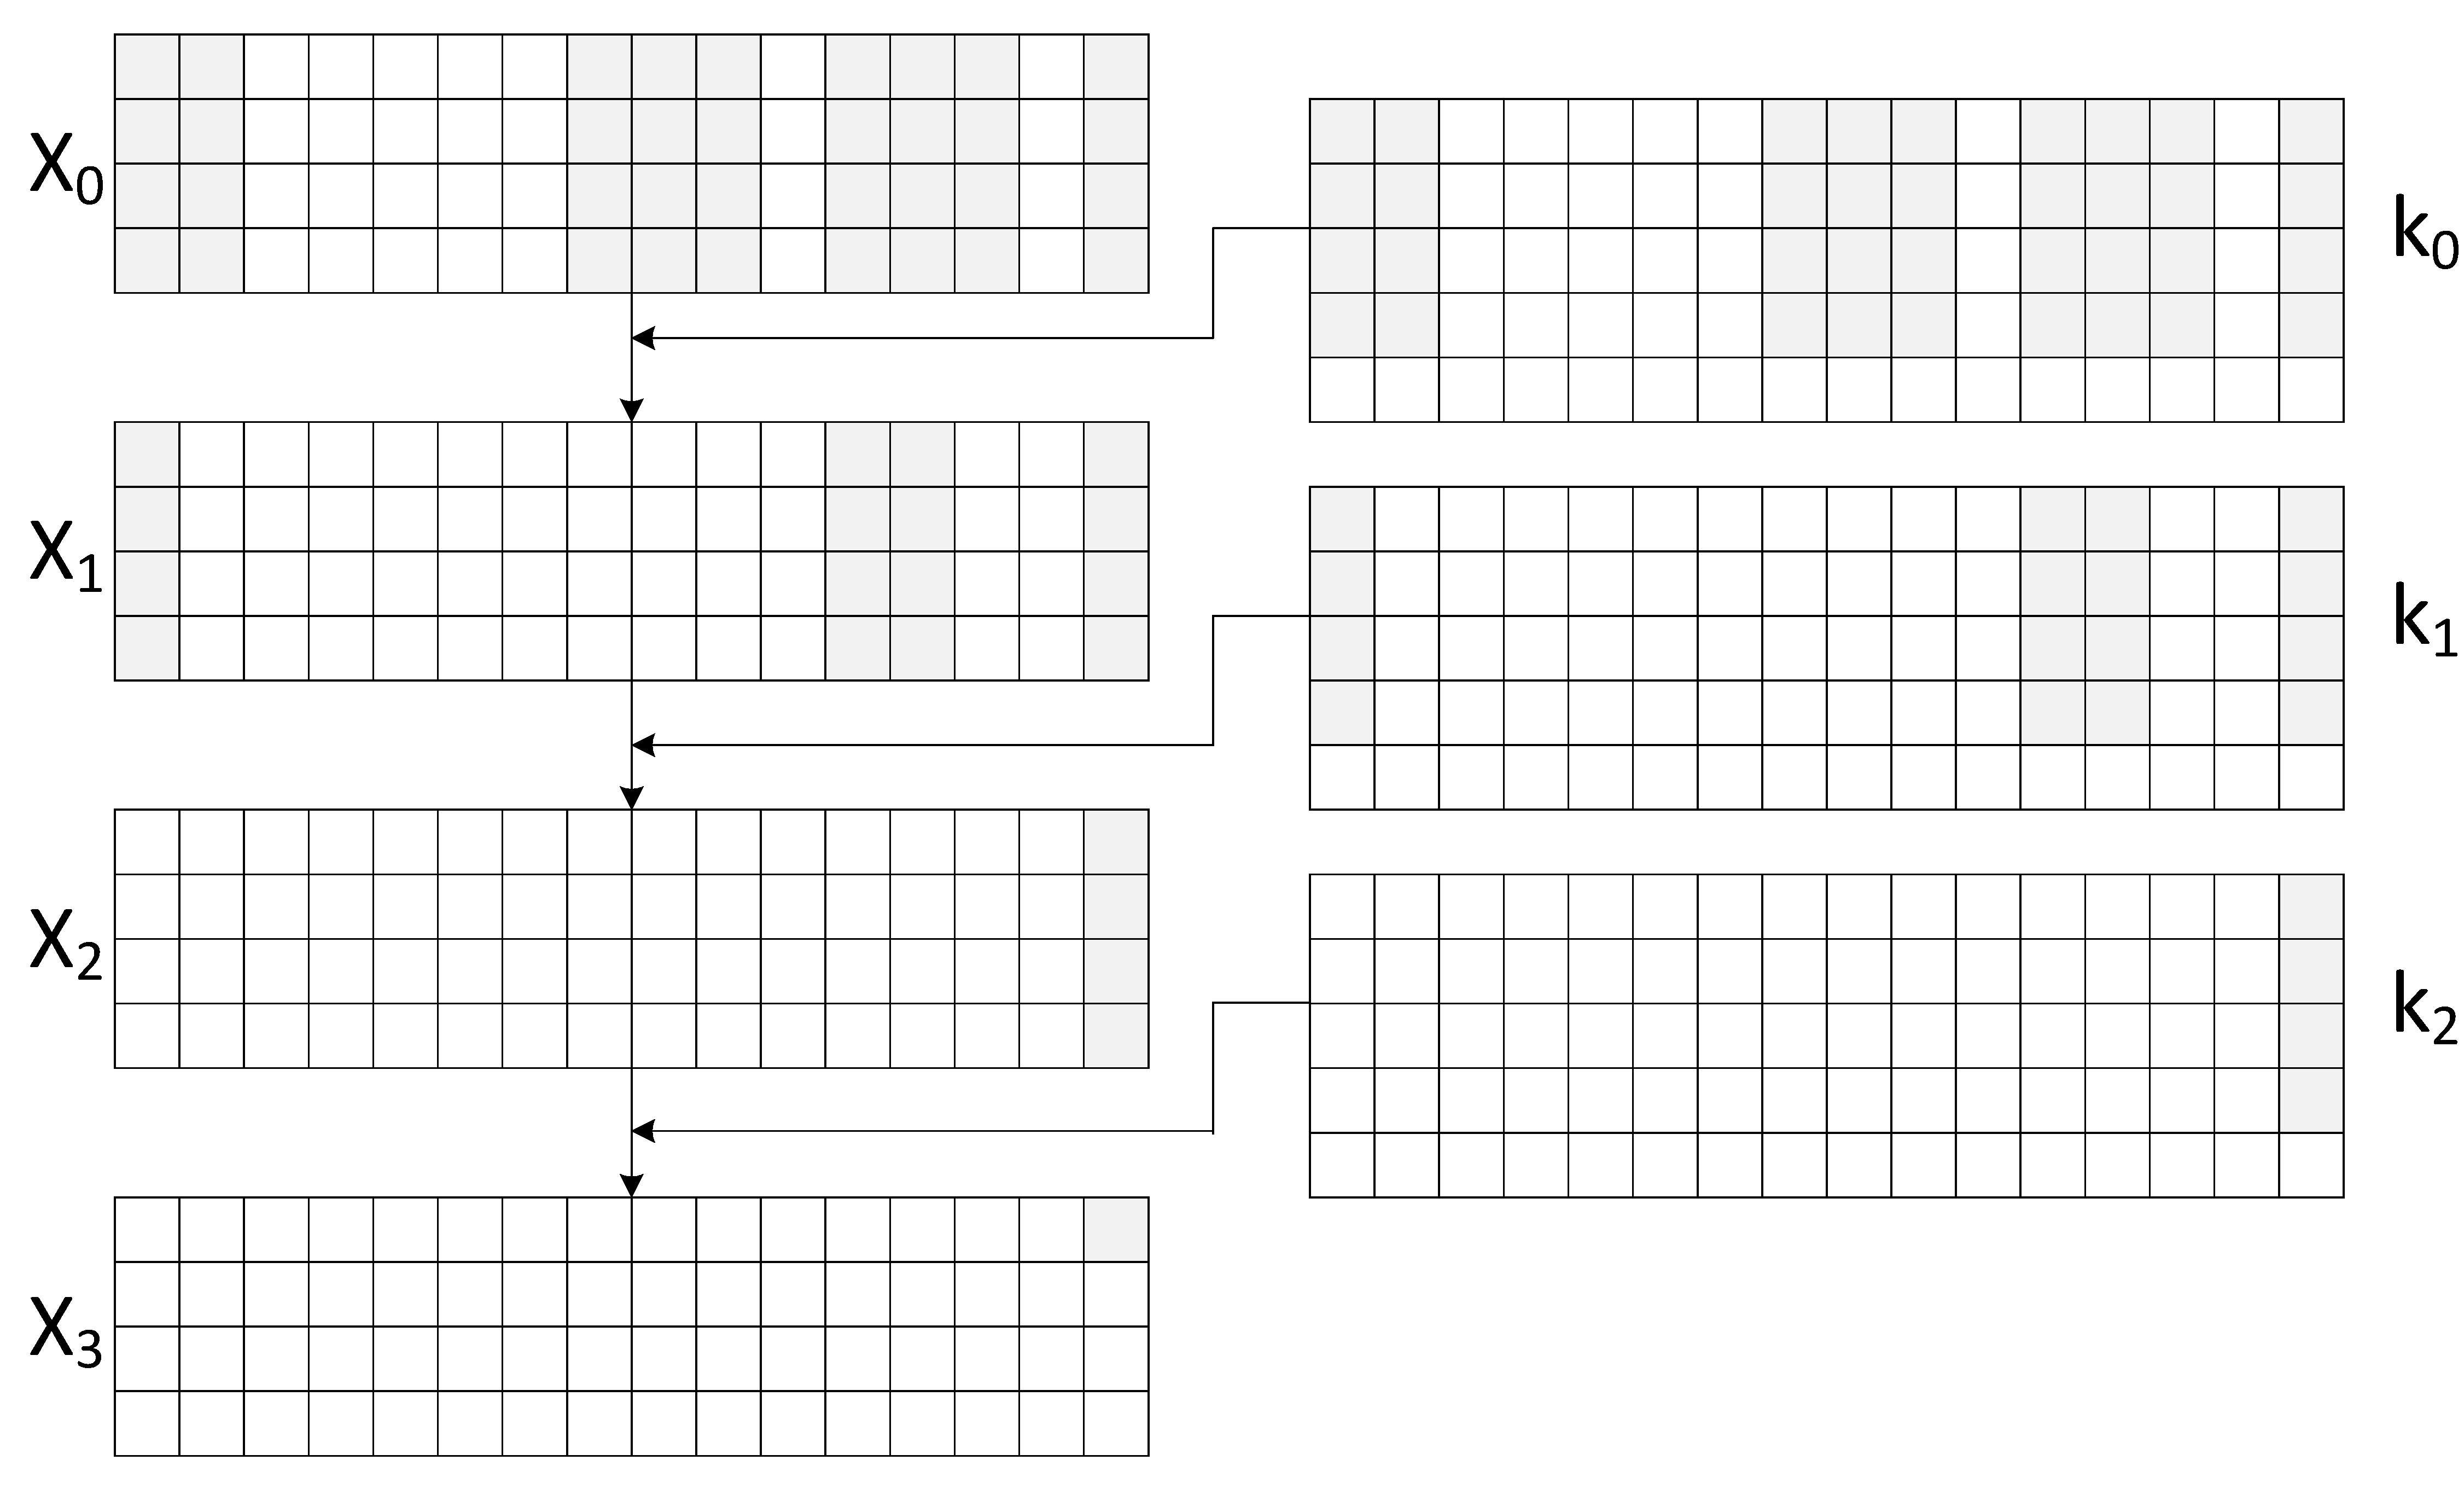
\includegraphics[height=5.5cm]{3KDP}
    \bicaption[fig:3KDP]{RECTANGLE-80的一条3轮路径}{RECTANGLE-80的一条3轮的计算路径和其密钥依赖路径}{3-round KDP}{A 3-round CP and KDP of RECTANGLE-80}
\end{figure}

由于PRESENT和RECTANGLE的结构、主密钥和分组长度都十分相似,在RECTANGLE的设计文档\citen{zhang2015rectangle}中作者比较了这两种加密方式的效率和安全性。
经过对以上4种密钥编排方案的AKI计算(见表\ref{tab:PREREC}),我们发现即使RECTANGLE的轮函数由于使用了bit-slice技术且仔细挑选了S盒而拥有更高的安全性和效率,但是它的AKI却在同轮比PRESENT少。
因此我们认为,PRESENT的密钥编排方案更加“配合”它的轮函数。

\begin{table}[tbp]
\centering
\begin{tabular}{c|cc|cc|cc|cc}
\hline
&\multicolumn{2}{c|}{RECTANGLE-80\quad}&\multicolumn{2}{c|}{PRESENT-80}&\multicolumn{2}{c|}{RECTANGLE-128\quad}&\multicolumn{2}{c}{PRESENT-128}\\
\hline
&$TKI$&\quad $AKI$&$TKI$&\quad $AKI$&$TKI$&\quad $AKI$&$TKI$&\quad $AKI$\\
$r=1$&4&4&4&4&4&4&4&4\\
$r=2$&20 & \textcolor{red}{18}&20 &20&20& \textcolor{red}{18}  &20 &20\\
$r=3$&56 &\textcolor{red}{42} &80 &\textcolor{red}{64}&56 &\textcolor{red}{44}  &84 &\textcolor{red}{77}\\
$r=4$&80 &\textcolor{red}{73} &80 &\textbf{80}&120 &\textcolor{red}{83} &128 &\textcolor{red}{125}\\
$r=5$&80 &\textbf{80}         &-  &-          &128 &\textcolor{red}{103} &128 &\textbf{128}\\
$r=6$&-&-&-&-&128 &\textcolor{red}{120}&- &-\\
$r=7$&-&-&-&-&128 &\textbf{128} &- &-\\
\hline
\end{tabular}
\bicaption[tab:PREREC]{PRESENT和RECTANGLE的AKI}{PRESENT-80/128和RECTANGLE-80/128的AKI}{AKI}{AKI of PRESENT and RECTANGLE}
\end{table}

另外,Zhang等人在设计RECTANGLE\citen{zhang2015rectangle}时单独分析了RECTANGLE的密钥编排方案(没有考虑轮函数),并称其80比特版本中,任意连续两轮的子密钥均依赖于所有80比特主密钥。
但是在结合轮函数和密钥编排方案两者的扩散程度的分析后我们发现,任意2,3,4轮的密钥依赖路径均没有完全包含整个密钥空间(密钥信息不足80比特),直到第5轮才得到完全的扩散。
类似地,在128比特版本中,作者称任意连续4轮子密钥均依赖于所有128比特子密钥,而在我们的结果中RECTANGLE-128使用了7轮才将密钥依赖路径扩散到整个密钥空间。

导致以上密钥信息泄露的其中一个主要的原因是密钥编排方案和轮函数两者扩散时的重叠。
这提醒了我们轮函数与密钥编排方案的扩散方式应该相辅相成,不能两者单独考虑。

\section{Midori和LED}
Midori是Banik等人\citen{banik2014midori}在2015年亚密会上提出的一种低能耗的轻量级SPN结构的分组密码。
Midori提供了两种不同的分组长度,分别为Midori-64(拥有64比特的分组长度)和Midori-128(128比特的分组长度)。
主密钥长度均为128比特。

Midori-64中,128比特的主密钥$K$被分为两个64比特的密钥$K_0$和$K_1$,即$K=K_0||K_1$。
白化密钥$WK=K_0\oplus K_1$,轮密钥$RK_i=K_{i\mbox{ mod }2}\oplus\alpha_i$,$0\leq i\leq 14$。
Midori-128中,白化密钥$WK=K$,轮密钥$RK_j=K\oplus\alpha_j$,$0\leq j\leq 18$。
其中$\alpha_i$是轮常数。

LED是由Guo等人\citen{Guo2011}在2011年提出的一个类AES的轻量级分组密码。
其分组长度为64比特,主密钥长度支持64比特和128比特。
LED的密钥编排方案十分简单,甚至可以说没有密钥编排方案——对于64比特长度的主密钥,$RK_i=K$,即轮密钥即为主密钥;
而对于128比特长度的主密钥,主密钥将会被分为两部分$K_0$和$K_1$,在加密时轮流使用$K_0$和$K_1$。

类似PRESENT和RECTANGLE,我们对LED和Midori计算了前几轮所有的密钥依赖路径的AKI,相关结果总结在

\begin{table}[htbp]
\centering
\begin{tabular}{c|cc|cc|cc|cc}
\hline
&\multicolumn{2}{c|}{Midori-64\quad}&\multicolumn{2}{c|}{Midori-128}&\multicolumn{2}{c|}{LED-64\quad}&\multicolumn{2}{c}{LED-128}\\
\hline
&$TKI$&\quad $AKI$&$TKI$&\quad $AKI$&$TKI$&\quad $AKI$&$TKI$&\quad $AKI$\\
$r=1$&25&\textcolor{red}{24}&13&\textcolor{red}{12}&64&64&64&64\\
$r=2$&85 &\textcolor{red}{72}&77 &\textcolor{red}{60}&64& \textbf{64}  &128 &\textbf{128}\\
$r=3$&128 &\textbf{128} &128 &\textcolor{red}{124}&- &- &- &-\\
$r=4$&- &- &128 &\textbf{128}&- &- &- &-\\
\hline
\end{tabular}
\bicaption[tab:MidoriLED]{Midori和LED的AKI}{Midori-64/128和LED-64/128的AKI}{AKI}{AKI of Midori and LED}
\end{table}

Midori和LED的设计者均摒弃了复杂的密钥编排方案,在Midori中只是简单的加了轮常数和白化密钥,而在LED中则几乎不存在常规意义上的“密钥编排方案”。
但有趣的是,即使这两种加密方式的编排方案看起来似乎更容易存在信息泄露,它们却能够在比PRESENT和RECTANGLE更少的轮数内达到AKI的理论最大值。
其中很大的原因在于这两者的轮函数扩散程度非常完善,其中LED更是能够在一轮就扩散到所有比特(即完全扩散)。
对于这种高扩散程度的轮函数,密钥编排方案的扩散程度便显得不那么重要。

\section{SIMON}
SIMON\citen{beaulieusimon}是Feistel结构轻量级密码的一个典型代表。
由于Feistel结构的特殊性,我们需要在确定轮函数依赖矩阵和密钥依赖矩阵时进行一定的变化。
SIMON的轮函数结构是典型的Feistel结构(见图\ref{fig:SIMON}),每轮中间状态的其中一半将会直接作为下一轮中间状态的另一半。
SIMON的密钥编排方案中轮密钥的生成也不是常见的迭代使用密钥扩展函数,而是从之前多轮的轮密钥生成一个新的轮密钥,见图\ref{fig:SIMONKey}。

\begin{figure}[htbp]
    \centering
    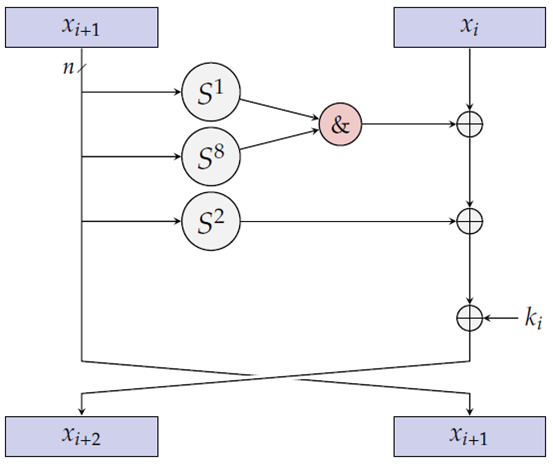
\includegraphics[width=5cm]{SIMON}
    \bicaption[fig:SIMON]{SIMON的轮函数结构}{SIMON轮函数的Feistel结构}{SIMON}{The Feistel structure of SIMON}
\end{figure}

\begin{figure}[htbp]
    \centering
    $$k_{i+m}=\begin{cases}
        c\oplus(z_j)_i\oplus k_i\oplus(I\oplus S^{-1})S^{-3}k_{i+1} & m=2\\
        c\oplus(z_j)_i\oplus k_i\oplus(I\oplus S^{-1})S^{-3}k_{i+2} & m=3\\
        c\oplus(z_j)_i\oplus k_i\oplus(I\oplus S^{-1})(S^{-3}k_{i+3}\oplus k_{i+1}) & m=4
    \end{cases}$$
    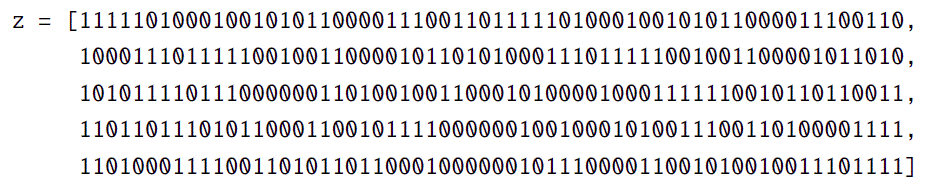
\includegraphics[width=10cm]{SIMONKey}
    \bicaption[fig:SIMONKey]{SIMON的密钥编排方案}{SIMON的密钥编排方案,其中$c$是常数,$z$是常数数组,$k_i,k_{i+1},k_{i+2}$是轮密钥,$S^j$表示循环左移$j$位,$I$表示不移位。}{SIMON}{The key schedule of SIMON, where $c$ is a constant and $z$ is a constant array, $k_i,k_{i+1},k_{i+2}$ is round keys, $S^j$ means left circular shifting by $j$ bits and $I$ means identity.}
\end{figure}

SIMON拥有很多不同的版本,有各自不同的分组长度和主密钥长度。
以最简单的分组长度32比特,密钥长度64比特,字(word)长度$n=16$比特,$m=4$为例,为了准确表示轮与轮中间状态的依赖关系,我们需要将中间状态设为$X_i=x_{i+1}||x_i$(见图\ref{fig:SIMON})。
由于SIMON的分组长度为32比特,这一点与前述的SPN结构密码无区别,但是在考虑该轮的AKI时,我们不能简单的取$X_i$中所有比特的路径中最小的AKI来计算——$X_i$和$X_{i+1}$中拥有共同的一块中间状态$x_{i+1}$,而这一块的路径必然是一样的,AKI也会相同。
因此在考虑某一轮的AKI时,我们应该事先确定好使用中间状态的某一部分。
考虑到经过一轮变换后,$X_1=x_2||x_1$,而$x_1$是明文中的一部分,因此取$x_1$作为AKI研究对象显然不合适。
因此,在考虑第$i$轮的AKI时,我们选择$X_i=x_{i+1}||x_i$中的$x_{i+1}$部分所有路径的最小AKI作为该轮的AKI。

在SIMON的密钥编排方案中,每一轮的轮密钥是由前$m$轮的轮密钥生成的。
因此,一轮轮密钥至少依赖于$mn$比特的轮密钥,则密钥依赖矩阵至少应为$\mathbb{N}^{mn\times mn}$。
在$n=16,m=4$的情况下,$k_{i+m}$依赖于$k_i,k_{i+1},k_{i+2},k_{i+3}$,因此我们设子密钥$WK_i=k_{i+3}||k_{i+2}||k_{i+1}||k_i$后,即可完整的表示出轮密钥之间的依赖关系。
可以看出这种情况下密钥依赖矩阵中,后$n$行表达出了真正的轮密钥的推导关系($k_{i+3}$的计算是由$WK_{i-1}$中的$mn$比特共同推出的),而前$(m-1)n$行中只有一个“1”(直接从上一个子密钥中搬来),只是为了保证$WK_i$中包含了足够推出$WK_{i+1}$的信息。

\begin{table}[htbp]
\centering
\begin{tabular}{c|c|c}
\hline
&\multicolumn{2}{c}{SIMON}\\
\hline
&$TKI$&$AKI$\\
\hline
$r=1$ & 1 & 1\\
$r=2$ & 4 & 4\\
$r=3$ & 10 & 10\\
$r=4$ & 20 & 20\\
$r=5$ & 34 & 34\\
$r=6$ & 50 & 50\\
$r=7$ & \textbf{64} & 63\\
$r=8$ & 64 & \textbf{64}\\
\hline
\end{tabular}
\bicaption[tab:SIMON]{SIMON的AKI}{SIMON的AKI}{AKI}{AKI of SIMON}
\end{table}

确定了两个矩阵的表示方法后,我们通过算法\ref{alg:AKI}的到SIMON的AKI,见表\ref{tab:SIMON}。
从表中可以看出,SIMON的TKI增长较慢,但前6轮都不存在密钥信息泄露,直到第7轮,密钥依赖路径的长度达到了$66>64$,但出现了3比特的密钥信息泄露,使得第7轮的AKI并没有达到理论最大值。


%# -*- coding: utf-8-unix -*-
%%==================================================
%% chapter01.tex for SJTU Master Thesis
%%==================================================

%\bibliographystyle{sjtu2}%[此处用于每章都生产参考文献]
\chapter{总结与讨论}
\label{chap:Con}
在本轮文中,我们给出了一个新的算法来解决黄佳琳提出的AKI问题,其不仅可以用来分析和确定密钥编排方案的扩散程度,也可以用来通过减少猜测集合的大小来优化如相关密钥攻击的密码攻击。
同事,我们也给出了一个新的方法来优化与重新设计一个没有密钥信息泄露的密钥编排方案。
为了展示我们提出的新方法的可行性和有效性,我们优化了对23轮TWINE-80的零相关攻击,并提出了一个新的对12轮RECTANGLE-128的中间相遇攻击,同时分别给出了新的密钥编排方案来帮助其抵抗这些攻击。

密钥依赖路径由于其与密钥编排方案无关,只与计算路径(轮函数)有关的特性,成为了使用AKI来为轮函数分析或设计密钥编排方案的重要途径。
在轮函数和轮密钥选择确定的前提下,某轮的某一比特的密钥依赖路径即随之确定,而此时不同的密钥编排方案就会带来不同的AKI,形成了物理实验中常见的“控制变量法”。
因此,要设计一个与轮函数相匹配的密钥编排方案,我们要做的就是找到一个AKI达到理论最大值的密钥编排方案。
为此,我们首先就需要一个能计算出精确AKI数值的算法(一个只能算出上界的算法只能用于攻击中优化猜测集合,而不能用来衡量编排方案的优劣)。
本文中使用了以密钥编排方案为基础构建流量网络图的方法,使用最大流问题解决了AKI问题。
进而我们需要反向思考,如何以“达到AKI理论最大值”为前提条件,找到符合条件的一个密钥编排方案。
本文中给出了一个对一个特定的子密钥集合设计一个相对较好的密钥编排方案的方法,但是其限制在于只能对一个集合达到AKI理论最大值,同时也无法保证是一个最优最简化的编排方案。
为了为轮函数设计一个更加普适的,能够对理论值超过主密钥长度的任何猜测集合都达到AKI理论最大值的密钥编排方案,我们就需要找到一个对不同的密钥依赖路径都有AKI最大的编排方案。
从单个集合设计的方案到能适应所有集合的方案的扩展十分困难,特别是当两个集合所设计出的方案大相径庭时,想要合并起来还要保持方案的简单性更加困难。
本文所提到的RECTANGLE-128的密钥编排设计主要是由于其依赖路径的特殊性(使所有依赖路径的AKI都达到最大的矩阵恰巧都为一个移位后的单位矩阵)才得到了一个普适的编排方案。
想要得到更加普遍的确定编排方案的方法,还需要进一步考虑其依赖矩阵的确定方式。

尽管,以我们有限的知识,我们只能给出一个基于给定的子密钥集合来寻找一个可能的、较小的密钥依赖矩阵的方法,我们仍然相信我们所构建的密码学与图论的“桥梁”将会帮助我们总结出一系列的科学的、理论的、完备的密钥编排方案设计方法与原则。


\appendix	% 使用英文字母对附录编号,重新定义附录中的公式、图图表编号样式
\renewcommand\theequation{\Alph{chapter}--\arabic{equation}}	
\renewcommand\thefigure{\Alph{chapter}--\arabic{figure}}
\renewcommand\thetable{\Alph{chapter}--\arabic{table}}
\renewcommand\thealgorithm{\Alph{chapter}--\arabic{algorithm}}

%% 附录内容,本科学位论文可以用翻译的文献替代。
%\include{tex/app_setup}
%\include{tex/app_eq}
%\include{tex/app_cjk}
%\include{tex/app_log}
\chapter{$K_t$和$K_b$的实际密钥信息集合}\label{AppendixA}
\textbf{$K_t$的实际密钥信息集合:}
\begin{table}[!h]
    \centering
\begin{tabular}{|l|l|l|l|l|l|l|l|}
\hline
$WK_{0}^{0}$&$WK_{0}^{1}$&$WK_{0}^{2}$&$WK_{0}^{3}$ &$WK_{0}^{4}$ &$WK_{0}^{5}$ &$WK_{0}^{6}$&$WK_{0}^{7}$\\
$WK_{0}^{8}$ &$WK_{0}^{9}$& $WK_{0}^{10}$& $WK_{0}^{11}$& $WK_{0}^{12}$&$WK_{0}^{13}$& $WK_{0}^{14}$& $WK_{0}^{15}$\\
$WK_{0}^{32}$ &$WK_{0}^{33}$ &$WK_{0}^{34}$&$WK_{0}^{35}$ &$WK_{0}^{36}$ &$WK_{0}^{37}$ &$WK_{0}^{38}$ &$WK_{0}^{39}$\\
$WK_{0}^{40}$&$WK_{0}^{41}$ &$WK_{0}^{42}$ &$WK_{0}^{43}$&$WK_{0}^{44}$&$WK_{0}^{45}$ &$WK_{0}^{46}$ &$WK_{0}^{47}$ \\
$WK_{0}^{64}$ &$WK_{0}^{65}$&$WK_{0}^{66}$&$WK_{0}^{67}$ &$WK_{0}^{68}$&$WK_{0}^{69}$&$WK_{0}^{70}$ &$WK_{0}^{71}$\\
$WK_{0}^{72}$ &$WK_{0}^{73}$ &$WK_{0}^{74}$ &$WK_{0}^{75}$&$WK_{0}^{76}$ &$WK_{0}^{77}$ &$WK_{0}^{78}$ &$WK_{0}^{79}$\\
$WK_{0}^{96}$&$WK_{0}^{97}$ &$WK_{0}^{98}$&$WK_{0}^{99}$ &$WK_{0}^{100}$ &$WK_{0}^{101}$&$WK_{0}^{102}$ &$WK_{0}^{103}$\\
$WK_{0}^{104}$&$WK_{0}^{105}$&$WK_{0}^{106}$&$WK_{0}^{107}$ &$WK_{0}^{108}$&$WK_{0}^{109}$ &$WK_{0}^{110}$ &$WK_{0}^{111}$\\
$WK_{1}^{0}$&$WK_{1}^{1}$&$WK_{1}^{2}$&$WK_{1}^{3}$&$WK_{1}^{4}$&$WK_{1}^{5}$&$WK_{1}^{6}$&$WK_{1}^{7}$\\
$WK_{1}^{64}$&$WK_{1}^{65}$&$WK_{1}^{66}$&$WK_{1}^{67}$&$WK_{1}^{68}$&$WK_{1}^{69}$&$WK_{1}^{70}$&$WK_{1}^{71}$\\
$WK_{1}^{72}$&$WK_{1}^{73}$&$WK_{1}^{74}$&$WK_{1}^{75}$&$WK_{1}^{76}$&$WK_{1}^{77}$&$WK_{1}^{78}$&$WK_{1}^{79}$\\
$WK_{2}^{0}$&$WK_{2}^{1}$&$WK_{2}^{2}$&$WK_{2}^{3}$&$WK_{2}^{4}$&$WK_{2}^{5}$&$WK_{2}^{6}$&$WK_{2}^{7}$\\
$WK_{2}^{64}$&$WK_{2}^{65}$&$WK_{2}^{66}$&$WK_{2}^{67}$&$WK_{2}^{68}$&$WK_{2}^{69}$&$WK_{2}^{70}$&$WK_{2}^{71}$\\
$WK_{2}^{72}$&$WK_{2}^{73}$&$WK_{2}^{74}$&$WK_{2}^{75}$&$WK_{2}^{76}$&$WK_{2}^{77}$&$WK_{2}^{78}$&$WK_{2}^{79}$\\
$WK_{3}^{0}$&$WK_{3}^{2}$&$WK_{3}^{3}$&$WK_{3}^{4}$&$WK_{3}^{6}$&$WK_{3}^{7}$&$WK_{3}^{64}$&$WK_{3}^{66}$\\
$WK_{3}^{67}$&$WK_{3}^{68}$&$WK_{3}^{70}$&$WK_{3}^{71}$&&&&\\
\hline
\end{tabular}
\end{table}
\newpage

\noindent
\textbf{$K_b$的实际密钥信息集合:}
\begin{table}[!h]
    \centering
\begin{tabular}{|l|l|l|l|l|l|l|}
\hline

$WK_{12}^{0}$&$WK_{12}^{1}$&$WK_{12}^{2}$&$WK_{12}^{3}$&$WK_{12}^{4}$&$WK_{12}^{5}$&$WK_{12}^{6}$\\
$WK_{12}^{7}$&$WK_{12}^{8}$&$WK_{12}^{9}$&$WK_{12}^{10}$&$WK_{12}^{11}$&$WK_{12}^{12}$&$WK_{12}^{13}$\\
$WK_{12}^{14}$&$WK_{12}^{15}$&$WK_{12}^{32}$&$WK_{12}^{33}$&$WK_{12}^{34}$&$WK_{12}^{35}$&$WK_{12}^{36}$\\
$WK_{12}^{37}$&$WK_{12}^{38}$&$WK_{12}^{39}$&$WK_{12}^{40}$&$WK_{12}^{41}$&$WK_{12}^{42}$&$WK_{12}^{43}$\\
$WK_{12}^{44}$&$WK_{12}^{45}$&$WK_{12}^{46}$&$WK_{12}^{47}$&$WK_{12}^{64}$&$WK_{12}^{65}$&$WK_{12}^{66}$\\
$WK_{12}^{67}$&$WK_{12}^{68}$&$WK_{12}^{69}$&$WK_{12}^{70}$&$WK_{12}^{71}$&$WK_{12}^{72}$&$WK_{12}^{73}$\\
$WK_{12}^{74}$&$WK_{12}^{75}$&$WK_{12}^{76}$&$WK_{12}^{77}$&$WK_{12}^{78}$&$WK_{12}^{79}$&$WK_{12}^{96}$\\
$WK_{12}^{75}$&$WK_{12}^{76}$&$WK_{12}^{77}$&$WK_{12}^{78}$&$WK_{12}^{79}$&$WK_{12}^{96}$&$WK_{12}^{97}$\\
$WK_{12}^{97}$&$WK_{12}^{98}$&$WK_{12}^{99}$&$WK_{12}^{100}$&$WK_{12}^{101}$&$WK_{12}^{102}$&$WK_{12}^{103}$\\
$WK_{12}^{104}$&$WK_{12}^{105}$&$WK_{12}^{106}$&$WK_{12}^{107}$&$WK_{12}^{108}$&$WK_{12}^{109}$&$WK_{12}^{110}$\\
$WK_{12}^{111}$&$WK_{11}^{0}$&$WK_{11}^{1}$&$WK_{11}^{2}$&$WK_{11}^{3}$&$WK_{11}^{4}$&$WK_{11}^{5}$\\
$WK_{11}^{6}$&$WK_{11}^{7}$&$WK_{11}^{8}$&$WK_{11}^{9}$&$WK_{11}^{10}$&$WK_{11}^{11}$&$WK_{11}^{12}$\\
$WK_{11}^{13}$&$WK_{11}^{14}$&$WK_{11}^{15}$&$WK_{11}^{72}$&$WK_{11}^{73}$&$WK_{11}^{74}$&$WK_{11}^{75}$\\
$WK_{11}^{76}$&$WK_{11}^{77}$&$WK_{11}^{78}$&$WK_{11}^{79}$&$WK_{10}^{0}$&$WK_{10}^{1}$&$WK_{10}^{2}$\\
$WK_{10}^{3}$&$WK_{10}^{4}$&$WK_{10}^{5}$&$WK_{10}^{6}$&$WK_{10}^{7}$&$WK_{10}^{8}$&$WK_{10}^{9}$\\
$WK_{10}^{10}$&$WK_{10}^{11}$&$WK_{10}^{12}$&$WK_{10}^{13}$&$WK_{10}^{14}$&$WK_{10}^{15}$&$WK_{10}^{72}$\\
$WK_{10}^{73}$&$WK_{10}^{74}$&$WK_{10}^{75}$&$WK_{10}^{76}$&$WK_{10}^{77}$&$WK_{10}^{78}$&$WK_{10}^{79}$\\
$WK_{9}^{8}$&$WK_{9}^{9}$&$WK_{9}^{10}$&$WK_{9}^{12}$&$WK_{9}^{13}$&$WK_{9}^{14}$&$WK_{9}^{72}$\\
$WK_{9}^{73}$&$WK_{9}^{74}$&$WK_{9}^{76}$&$WK_{9}^{77}$&$WK_{9}^{78}$&&\\
\hline
\end{tabular}
\end{table}


\backmatter	% 文后无编号部分 

%% 参考资料
\printbibliography[heading=bibintoc]

%% 致谢、发表论文、申请专利、参与项目、简历
%% 用于盲审的论文需隐去致谢、发表论文、申请专利、参与的项目
\makeatletter

%%
% "研究生学位论文送盲审印刷格式的统一要求"
% http://www.gs.sjtu.edu.cn/inform/3/2015/20151120_123928_738.htm

% 盲审删去删去致谢页
%\ifsjtu@review\relax\else
  %# -*- coding: utf-8-unix -*-
\begin{thanks}

本人的学位论文是在我的导师来学嘉教授的指导下完成的。
感谢来教授用丰富的专业知识指导我完成对密钥编排方案的深度探究,从开题到构思、撰写和定稿,来教授都给了我莫大的帮助。
来教授渊博的学识与对学术兢兢业业的态度,激励着我向信息安全领域进一步求学的信念。

感谢闫海伦学姐的指导,在与闫海伦学姐讨论中,我学到的不仅是丰富的专业知识,还学到了作为一个研究者应有的态度和努力。

最后感谢我的家人在此期间给予我的包容、关爱和鼓励,以及所有陪我一路走来的同学和朋友,
正是由于他们的支持和照顾,我才能安心学习,并顺利完成我的学业。

\end{thanks}
 	  %% 致谢
%\fi

\ifsjtu@bachelor
  % 学士学位论文要求在最后有一个英文大摘要,单独编页码
  \pagestyle{biglast}
  %# -*- coding: utf-8-unix -*-
\begin{bigabstract}
The low diffusion of a simplified key schedule in block ciphers is usually responsible for many attacks.
    Huang \emph{et al.} gave conceptions on Key Information, especially the Actual Key Information (AKI), which successfully illustrated and quantified the method to evaluate the diffusion of a key schedule.
    However, the algorithm used to calculate AKI proposed by Huang \emph{et al.} cannot be used to determine the weakness or further make an optimization of a key schedule since it cannot give an accurate value of AKI.
    In this paper, we successfully solve the AKI problem by our AKI - Minimum Cut Algorithm based on the well-known Max-flow problem in Graph Theory,
    and further give a method to design a key schedule which offers better security with less or without Key Information leakage.
    As applications, we optimize the zero-correlation attack on 23-round TWINE-80 and find a new meet-in-the-middle attack on 12-round RECTANGLE-128,
    and respectively give a new dependency matrix for TWINE-80 and an optimized key schedule for RECTANGLE-128, which makes both of them stronger against these attacks.

A key schedule is an algorithm that expands a relatively short master key to a large expanded key as round keys used in encryption and decryption algorithms.
When it comes to block ciphers, the key schedules are often simplified due to implementation considerations and cause weakness that can be exploited in many attacks, especially for lightweight block ciphers since their schedule are designed based on not only the security but also the effciency of software and hardware.
Key schedules like that of PRESENT\citen{Bogdanov}, RECTANGLE\citen{zhang2015rectangle}, TWINE\citen{Suzaki_2013} and LBlock\citen{Wu_2011} are round-by-round iterations with low diffusion;
Key schedules like that of SIMON and SPECK\citen{beaulieusimon} have simple permutations or linear operations with low diffusion.
Some ciphers like LED\citen{Guo2011} do not even have a key schedule, and just use master keys directly in each round.
Those key schedules are simple and efficient but responsible for many attacks, especially related-key attack\citen{biham1994new,Biryukov2009,Ko2004} and meet-in-the-middle attack\citen{diffie1977special,Biryukov2015,Bogdanov2011}.

In order to illustrate and quantify the diffusion and the detailed weakness which should be responsible for the genetic attacks, Huang \emph{et al.} gave conceptions on Key Information in \citen{huang2014revisiting}, including Computation Path, Key Dependency Path and Actual Key Information, which vividly described the diffusion of a key schedule. 
Taking use of the Key Information leakage of key schedules, Huang \emph{et al.} derived meet-in-the-middle attacks on 40-round SHACAL-2\citen{Handschuh2002} and 25-round XTEA\citen{Needham1997} in \citen{huang2014revisiting} and further proposed an algorithm in \citen{Huang_2014} which could give a reasonable upper bound of the AKI of a key schedule.
However, to design a key schedule which offers more security in Key Information, an accurate value of AKI is required and a method or principle for such a design is essential.

\noindent
\textbf{Our Contribution}. In this paper, we demonstrate a polynomial algorithm solving the AKI problem based on Graph Theory, building a "bridge" between key schedules and flow networks.
We describe the method solving AKI problem from the highly simplied version problem of 1-round AKI, and prove the equivalence between 1-round schedule and bipartite graph.
Further, we introduce the Max-flow Min-cut Theorem and give our AKI - Mimimum Cut Algorithm.
A theoretical proof of the correctness of our algorithm is also included.
By calculating the accurate AKI, we optimize the zero-correlation attack on 23-round TWINE-80 and derive a new meet-in-the-middle attack on 12-round RECTANGLE-128.

Meanwhile, taking use of the "bridge" between key schedules and flow networks we build, we give a greedy algorithm which can generate a new schedule (presented in dependency matrix) from a given subkey set without Key Information leakage.
Based on this algorithm, we respectively give a new matrix for TWINE-80 against the zero-correlation attack and a new key schedule for RECTANGLE-128 which makes any meet-in-the-middle attack on more than 8 rounds impossible.

The source code of the algorithms mentioned above is available \href{https://github.com/KirisameNanami/AKI-Algorithms}{here}.

In order to determine the existance of Key Information leakage, there are several algorithms to compute AKI.
Huang has given an automatic detection tool which includes the calculation of AKI in \citen{Huang_2014}, but the algorithm was a greedy algorithm, which means that it could only give a possible upper bound of AKI.
Also, the Automatic Search of Key-Bridging Technique\citen{dunkelman2010improved} proposed by Lin \emph{et al.} in \citen{lin2016automatic} could also find an upper bound of AKI (since a key bridge is exactly 1-bit leakage of Key Information).
However, neither of the two algorithm could compute the accurate value of AKI (a counterexample will be provided in following sections), which made them a tool for generating an attack such as meet-in-the-middle attack \citen{diffie1977special}, but not for evaluating the safety of a key schedule.
Also, the low efficiency of both of the algorithms (usually several minutes for a single subkey set) limit the application to a whole key schedule, since we have to examine the KDPs from all the internal bits.
In this paper, we will demonstrate our AKI - Minimum Cut Algorithm based on Graph Theory which can get the accurate value of AKI.
This AKI algorithm is based on graph theory, aims at transform the key schedule (represented by the dependency matrix $M$) and a subkey bits set $K$ to a directed flow graph $G_f(E,V,c)$.
Algorithm .~\ref{alg:const} is used to construct such graph.
Briefly speaking, besides the two completely new vertex $s$ and $t$, we construct two vertex $u_{in},u_{out}$ for each bit which is or is depended by the bits in $K$ according to the key schedule $M$, and connect them from $u_{in}$ to $u_{out}$ with a capacity of 1.
All the other edge has its capacity of infinity, and there're three kinds of those edges:
\begin{enumerate}
    \item Edge from $s$ to $u_{in}$ where $u$ is in first round,
    \item Edge from $u_{out}$ to $t$ where $u\in K$,
    \item Edge from $u^{b}_{out}$ to $u^{b'}_{in}$ where $b$ and $b'$ are in two consecutive rounds and $b'$ depends on $b$ according to the key schedule.
\end{enumerate}

For a subkey set $K$ and a dependency matrix $M$ of a $n$-bit key schedule, let $R$ be the maximum round on which bits in $K$ are.
Then the graph $G_f$ constructed by Algorithm.~\ref{alg:const} will have at most $2nR$ vertices (each bit has two vertices and there are at most $R\cdot n$ bits) and $n+|K|+nR+n^2R$ edges (consider the situation that $M$ is a full matrix).
Currently there are many algorithms to solve Max-flow problem. The Push Relabel Algorithm (with highest label node selection rule) has its performance of $\mathcal{O}(V^2\sqrt{E})$ in time complexity, where $V$ and $E$ stands for the number of vertices and edges, respectively.
Hence, the time complexity for our AKI - Minimum Cut algorithm will be $\mathcal{O}((2nR)^2\sqrt{n+|K|+nR+n^2R})=\mathcal{O}(n^3R^{2.5})$, which is polynomial.
It guarantees that for most encryption methods, our algorithm can terminate in seconds.

Since the AKI-set plays the same role with the subkey set $K$ in Key Information, once there exists a leakage of Key Information, the complexity of an attack based on a guessing set $K$ (usually with a distinguisher whose input/output is the set which $K$ is generated from) will be easily reduced by replacing $K$ by its AKI-set $K'_0$.
In this paper, we will introduce two applications based on Key Information leakage.

After we quantify the key schedule with a flow network constructed by Algorithm.~\ref{alg:const}, we can further consider how to design a key schedule with the best performance in terms of AKI.
Theoretically, for a key schedule with a $n$-bit master key and a subkey set $K$, if $|K|\geq n$, there must exist a key schedule with its dependency matrix $M$ which makes the AKI of $K$ be $n$.
This conclusion is trivial since a full matrix (all the cells are 1) $M_{full}$ obviously meet the requirments.
However, such a full matrix $M_{full}$ cannot be used in practical as a dependency matrix of a key schedule.
Hence, we need to find a matrix with the number of '1's as small as possible.

In this paper, we give a new algorithm to give the accurate value of AKI defined by Huang \emph{et al.}, which can be used not only to evaluate and determine the diffusion of a key schedule, but also to optimize the subkey set used in attacks like related-key attack.
We also gives a new method to optimize and re-design a key schedule without Key Information leakage.
To demonstrate the usefulness of those methods, we optimize the zero-correlation attack on 23-round TWINE-80 and generate a new meet-in-the-middle attack on 12-round RECTANGLE-128,
and respectively give new key schedules for both of them which make them secure enough against their attacks.

Although, to the best of our knowledge, we only provide the method of finding a possible, relatively small dependency matrix on a certain subkey set,
we still believe that the "bridge" we built between key schedules and flow networks will work further in summarizing a scientific, theoretical and complete serial of principles on designing the key schedule for a round function.

\end{bigabstract}

\else
  % 盲审论文中,发表学术论文及参与科研情况等仅以第几作者注明即可,不要出现作者或他人姓名
  \ifsjtu@review\relax
    \include{tex/pubreview}
    \include{tex/projectsreview}  
  \else
    \include{tex/pub}	      %% 发表论文
    \include{tex/projects}  %% 参与的项目
  \fi
\fi

% \include{tex/patents}	  %% 申请专利
% \include{tex/resume}	  %% 个人简历

\makeatother

\end{document}
